\documentclass[times, utf8, zavrsni, numeric]{fer}
\usepackage{booktabs}
\usepackage{listingsutf8}
\usepackage[final]{pdfpages}
\usepackage[titletoc,page]{appendix}
\captionsetup[lstlisting]{position=bottom}
\addto\captionsenglish{%
  \renewcommand{\figurename}{Slika}%
  \renewcommand{\contentsname}{Sadržaj}
  \renewcommand{\appendixname}{Dodatak}
  \renewcommand\appendixpagename{Dodaci}
  \renewcommand\tablename{Tablica}
  \renewcommand\bibname{Literatura}
  \renewcommand{\lstlistingname}{Primjer}
}
\usepackage{listings}
\usepackage{color}

\definecolor{dkgreen}{rgb}{0,0.6,0}
\definecolor{gray}{rgb}{0.5,0.5,0.5}
\definecolor{mauve}{rgb}{0.58,0,0.82}

\lstset{frame=tb,
  language=Java,
  aboveskip=3mm,
  belowskip=3mm,
  showstringspaces=false,
  columns=flexible,
  captionpos=b,
  basicstyle={\small\ttfamily},
  numbers=none,
  numberstyle=\tiny\color{gray},
  keywordstyle=\color{blue},
  commentstyle=\color{dkgreen},
  stringstyle=\color{mauve},
  breaklines=true,
  breakatwhitespace=true,
  tabsize=3
}
\lstset{
    literate=%
    {ć}{{\'c}}1
    {č}{{\v{c}}}1
    {đ}{{\dj{}}}1
    {š}{{\v{s}}}1
    {ž}{{\v{z}}}1
    {Ć}{{\'C}}1
    {Č}{{\v{C}}}1
    {Đ}{{\DJ{}}}1
    {Š}{{\v{S}}}1
    {Ž}{{\v{Z}}}1
}
\begin{document}

% TODO: Navedite broj rada.
\thesisnumber{4573}

% TODO: Navedite naslov rada.
\title{Obrada podataka tehnologijom Apache Spark}

% TODO: Navedite vaše ime i prezime.
\author{Martin Matak}

\maketitle

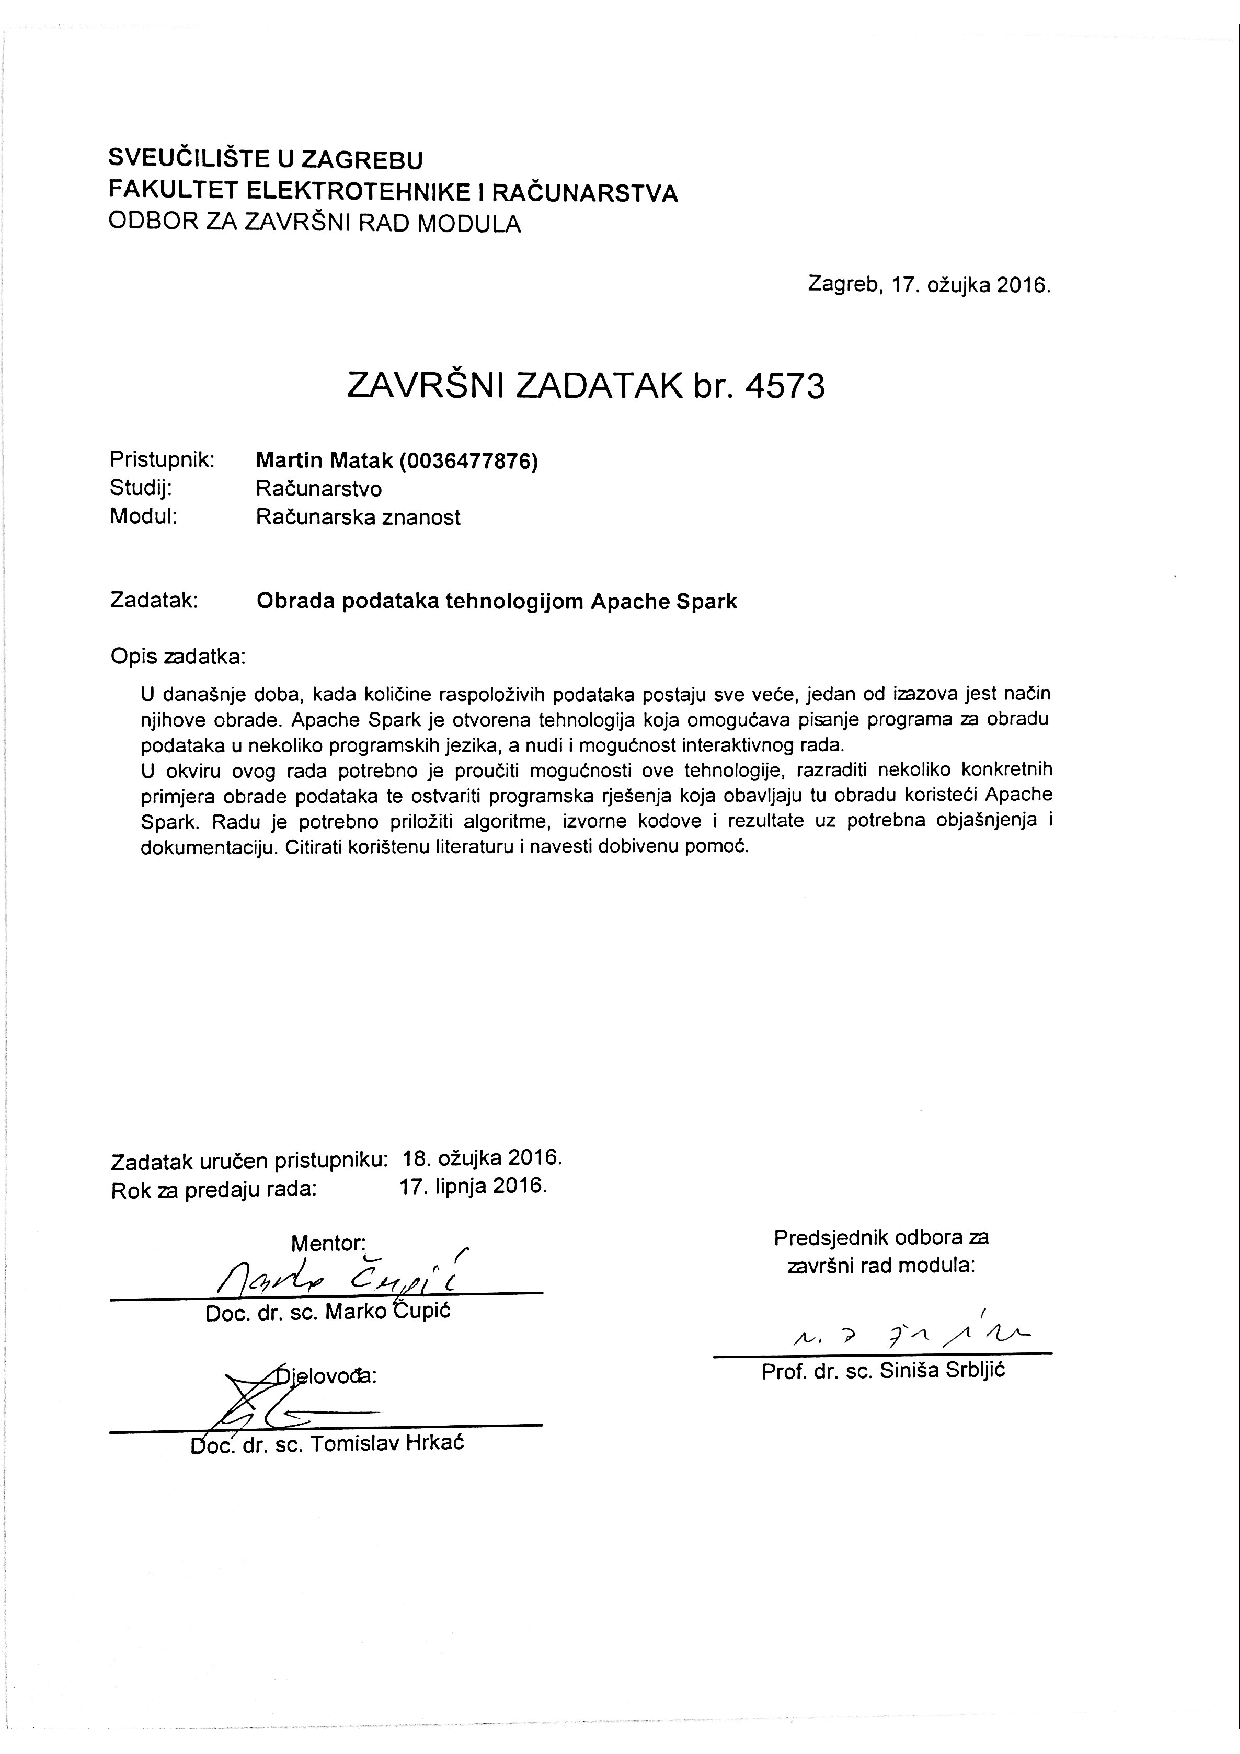
\includepdf[pages=-]{img/izvornik.pdf}

% Dodavanje zahvale ili prazne stranice. Ako ne želite dodati zahvalu, naredbu ostavite radi prazne stranice.
\zahvala{Zahvaljujem se doc. dr. sc. Marku Čupiću na mentorstvu, pomoći i savjetima pruženim pri pisanju ovog završnog rada.}

\tableofcontents

\chapter{Uvod}
Skoro pa svaka osoba danas posjeduje mobilni uređaj, a neke osobe posjeduju i više njih. Pametni mobilni uređaji postaju neizostavan dodatak svakog modernog čovjeka. Prošlo je vrijeme kada su mobilni uređaji jedino služili za pozive i SMS poruke. Današnji mobilni uređaji imaju puno više mogućnosti. Osim što je zadržana funkcionalnost uspostavljanja poziva i slanja poruka, postoji mogućnost povezivanja na internet, orijentaciju u prostoru, mjerenje brzine itd. Da bi sve te stvari bile moguće, većina današnjih mobilnih uređaja u sebi sadrži senzore poput akcelerometra, barometra, senzora svijetlosti, žiroskopa, geomagnetskog senzora itd.

Pretpostavimo da je mobilni uređaj spojen na internet i da svakih nekoliko sekundi pošalje vrijednost koju u tom trenutku mjeri pojedini senzor. U samo jednom danu može se skupiti dosta podataka. A što kada to ne bi radili za jedan uređaj nego za sve izdane uređaje nekog modela? Količina podataka bi jako brzo narasla.

Kako količina podataka postaje sve veća, dolazimo do pojma \emph{Velika količina podataka} \engl{Big Data}. U današnje vrijeme postoji više podataka u digitalnom obliku nego što ih je ikada bilo. Jedan od zanimljivijih izazova je kako ih djelotvorno obraditi i zaključiti nešto iz toga, odnosno kako od te velike količine podataka doći do nekih pametnih zaključaka i nešto novo naučiti.

Tehnologija \emph{Apache Spark} je tehnologija otvorenog koda \engl{open source} koja omogućava pisanje programa za obradu podataka u tri programska jezika: Javi, Pythonu i Scali. Dodatno, postoji i mogućnost interaktivnog rada. \\
U okviru ovog rada proučeni su neki djelovi ove tehnologije, razrađeno je nekoliko konkretnih primjera obrade podataka te ostvareno programsko rješenje koja obavljaju tu obradu koristeći tehnologiju \emph{Apache Spark}.

Ostatak rada organiziran je kako slijedi. U poglavlju 2 navedeni su osnovni gradivni elementi te su ukratko opisani. U poglavlju 3 opisana je osnovna struktura aplikacije. U poglavlju 4 obrađen je algoritam \emph{PageRank} te je uveden pojam dijeljenih varijabli. U poglavlju 5 nalazi se zaključak ovog rada. 

Svi primjeri su napisani u programskom jeziku Java.

\chapter{Osnovni gradivni elementi}
Tehnologija \emph{Apache Spark} je pisana u programskom jeziku Scala i izvršava se na \emph{Javinom virtualnom stroju} (engl. \emph{Java Virtual Machine}, kratica JVM). Instalacija na osobno računalo je objašnjena u dodatku \ref{ch:instalacijaSpark}. Opisi nekih direktorija i datoteka koje se dobiju instalacijom dani su u tablici \ref{tbl:installPackage}. Zanimljivo je spomenuti da postoji interaktivna ljuska \emph{Spark shell}, ali isključivo za programske jezike Python i Scala. Datoteke u direktoriju \emph{bin} služe upravo za to. Budući da je ovaj rad ograničen isključivo na programski jezik Java, a u ovom trenutku takva interaktivna ljuska još ne postoji, interaktivna ljuska nije detaljnije obrađena. Više informacija o ljusci moguće je pronaći u \cite{learningSpark}.

\begin{table}[htb]
\caption{Dio datoteka i direktorija dobivenih instalacijom.}
\label{tbl:installPackage}
\centering
\begin{tabular}{l p{8cm}}
\hline
Datoteka ili direktorij & Opis \\
\hline
\emph{bin} & Sadrži izvršive datoteke koje se koriste za interaktivni rad s tehnologijom \emph{Apache Spark}.\\
\emph{core, streaming, python, ...} & Sadrži glavne komponente tehnologije. \\
\emph{README.md} & Sadrži kratke instrukcije za upoznavanje s tehnologijom.\\
\emph{examples} & Sastoji se od nekoliko jednostavnih primjera koje pomažu korisniku da se uhoda i što bezbolnije nauči koristiti programsko sučelje koje tehnologija pruža. \\
\hline
\end{tabular}
\end{table}

Osnovna programska apstrakcija s kojom tehnologija \emph{Apache Spark} radi je \emph{otporni raspodijeljeni skup podataka} (engl. \emph{resilient distributed dataset}, kratica RDD) \cite{workingSets}.
Atribut \emph{otporni} znači da se može ponovno rekonstruirati u slučaju da se particija uništi. Cijeli skup podataka je podijeljen u odgovarajući broj particija (koji se može, a i ne mora ručno zadati). Podatci su podijeljeni u particije na način da im je lakše i brže pristupati te ih obrađivati. Dobra praksa je imati 2-4 particije po raspoloživom procesoru na grozdu. \emph{Raspodijeljeni} znači da je to skup podataka koji se nalazi na računalima (jednom ili više njih) i moguće ga je paralelno obrađivati. \emph{Skup podataka} znači da predstavlja kolekciju podataka. Tehnologija \emph{Apache Spark} nudi bogato programsko sučelje za rad s takvim skupovima podataka.

\vspace{5mm}
\begin{figure}[htb]
\centering
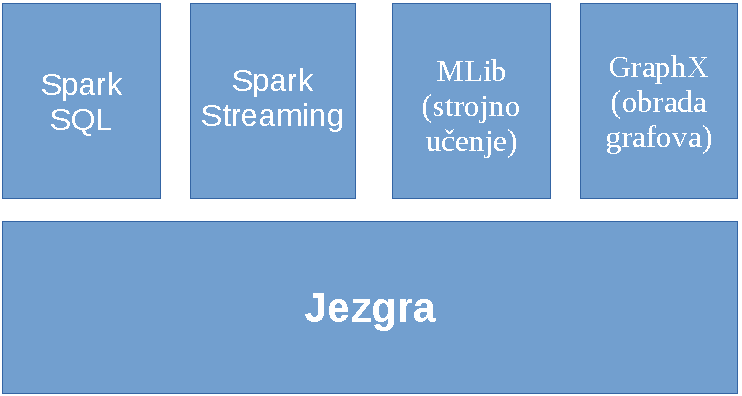
\includegraphics[width=10cm]{img/gradivniElementiCropped.pdf}
\caption{Osnovni elementi tehnologije \emph{Apache Spark}.}
\label{fig:spark-stack}
\end{figure}


Tehnologija se sastoji od nekoliko ključnih elemenata koji su u nastavku nabrojani i kratko opisani. Detaljnije objašnjenje nalazi se u službenoj dokumentaciji \cite{officialDocumentation}. Slika \ref{fig:spark-stack} prikazuje osnovne elemente tehnologije \emph{Apache Spark}.

Jezgra je odgovorna za upravljanje rasporedom zadataka \engl{task scheduling}, upravljanje memorijom, oporavak od pogreške i još mnogo toga. Jezgra je mjesto gdje se definira sučelje za otporni raspodijeljeni skup podataka. Ovdje se definiraju sve transformacije i akcije\footnote{Transformacije i akcije obrađene su u potpoglavlju \ref{RDD}}.   

SparkSQL omogućuje rad s bilo kakvim strukturiranim podatcima, primjerice \emph{JSON}. Također, nudi i mogućnost izvršavanja \emph{SQL} naredbi. Nalazi se u ovoj tehnologiji od njene verzije 1.0. Njegova starija zamjena bio je Shark koji je bio projekt na Berkeleyu. On je radio potrebne modifikacije na Apache Hive-u kako bi se mogao vrtiti na Sparku.

Spark Streaming je komponenta koja je zadužena za rad s tokovima podataka. Ti tokovi podataka mogu biti podatci koji nastaju u realnom vremenu. Primjer toka podataka u realnom vremenu mogu biti \emph{log} datoteke koje nastaju na nekom web-poslužitelju koji je u produkciji. Sučelje koje Spark Streaming pruža slično je sučelju koje pruža i otporni raspodijeljeni skup podataka, a to omogućava programerima da se brzo nauče koristiti ovu komponentu. 

MLib koristi se za postupke strojnog učenja. Omogućava širok spektar algoritama za strojno učenje poput klasifikacije, regresije i  grupiranja. Također nudi funkcionalnost koja omogućava evaluaciju modela i učitavanje podataka. Nudi i jednostavnije algoritme strojnog učenja poput optimizacijskog algoritma gradijentnim spustom. Sve mogućnosti ove komponente napravljene su na način da se mogu skalirati na cijeli grozd.

GraphX je biblioteka za obradu grafova (npr. graf prijatelja na društvenoj mreži). Poput komponenti SparkSQL i Spark Streaming,  ova komponenta također ima sučelje koje je vrlo slično sučelju za rad s otpornim raspodijeljenim skupovima podataka. Omogućava kreiranje usmjerenih grafova s proizvoljnim vrijednostima na bridovima i vrhovima. U sebi sadrži biblioteku popularnih algoritama za rad s grafovima, a jedan od takvih algoritama je i algoritam \emph{PageRank} koji je opisan u potpoglavlju \ref{algoritamPageRank}.

\chapter{Prvi programi}
U ovom poglavlju opisano je kako napisati osnovni program koristeći tehnologiju \emph{Apache Spark}. Također je opisano i od čega se takav program sastoji te koja je uloga pojedine komponente programa. Primjer koji se obrađuje je primjer \ref{lst:brojanjeRijeci}, a svodi se na jednostavan algoritam brojanja riječi.

\section{Postavljanje temelja}
\subsection{Osnovni elementi aplikacije}
Općenito govoreći, svaka se Spark aplikacija sastoji  od nekoliko komponenata. Prva komponenta koju ćemo spomenuti je program koji se izvršava - onaj čija je \texttt{main} metoda pokrenuta, odnosno onaj koji pokreće obradu podataka. Taj program naziva se pozivajući program \engl{driver}. Pozivajući program vrši obradu podataka kroz  \emph{SparkContext}.

\begin{figure}[htb]
\centering
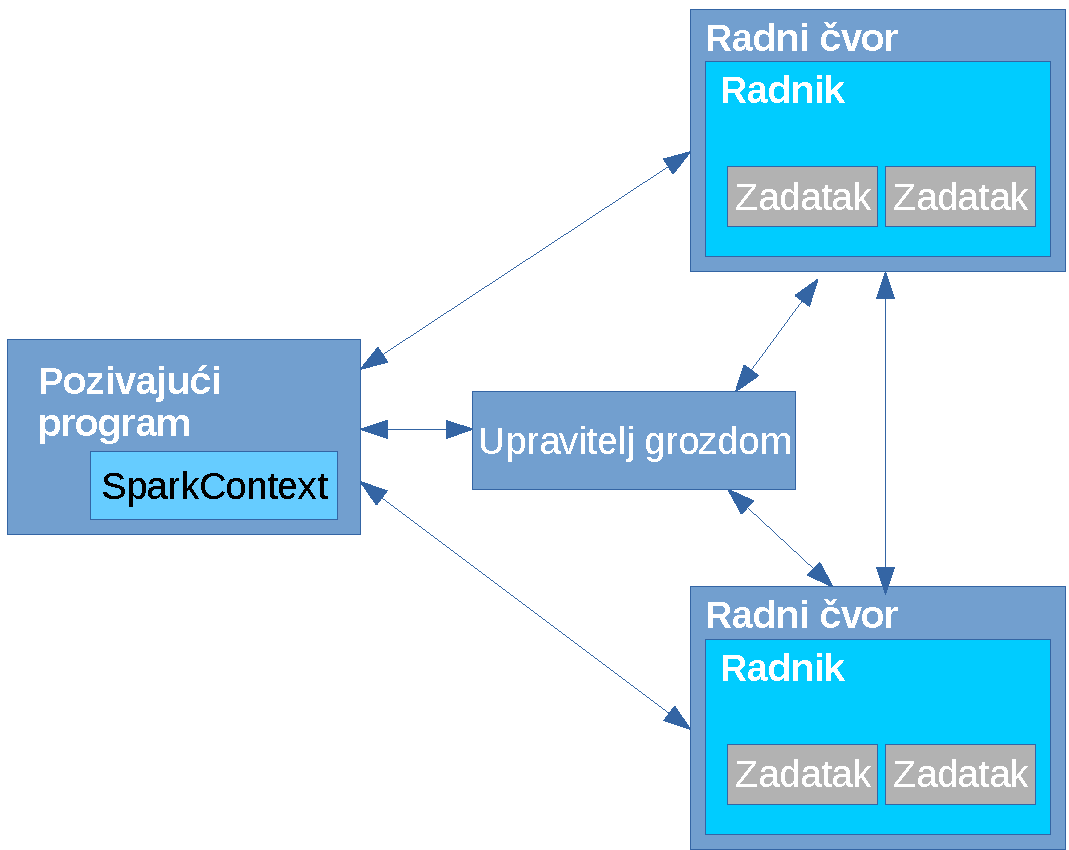
\includegraphics[scale=0.55]{img/elementiAplikacijeCropped.pdf}
\caption{Prikaz elemenata aplikacije.}
\label{fig:cluster-overview}
\end{figure}

Budući da je tehnologija \emph{Apache Spark} namijenjena za paralelnu obradu podataka, postoje još dvije komponente koje pridonose upravo tome. Pojedino računalo u \emph{grozdu} \engl{cluster} naziva se \emph{radnim čvorom} \engl{worker node}, a proces koji se izvršava na pojedinom računalu naziva se \emph{radnik} \engl{executor}. Dozvoljeno je da \emph{radnici} međusobno komuniciraju. U cijeloj priči može, a i ne mora eksplicitno biti uključen \emph{upravitelj grozdom} \engl{cluster manager}.
Opisana struktura prikazana je na slici \ref{fig:cluster-overview}.

\subsection{Korištenje tehnologije Apache Spark kroz programski jezik Java}
Kako bi mogli pisati Spark programe u programskom jeziku Java, potrebno je imati biblioteke koje nisu sastavni dio platforme JDK.
Jedna mogućnost je potražiti ih na internetu te ih ručno dohvatiti, raspakirati i uvesti u projekt. Druga mogućnost je koristiti automatizaciju razvojnog ciklusa. Jedan od alata koji to omogućuje je Maven. Za postavljanje i instalaciju Mavena konzultirati poveznicu \footnote{\url{https://maven.apache.org/install.html}} i knjigu \cite{marcupic}. Za vrijeme pisanja ovog rada, najnovija verzija Sparka je 1.6.1, a odgovarajuće Maven koordinate su:
\begin{lstlisting}[language=bash, basicstyle=\small]
groupId = org.apache.spark
artifactId = spark-core_2.10
version = 1.6.1
\end{lstlisting}

Odgovarajuća \texttt{pom.xml} datoteka prikazana je u dodatku \ref{ch:datotekapomXML}.
Jednom kada je \texttt{pom.xml} datoteka namještena i projekt uspješno povezan s bibliotekom \texttt{spark-core}, sve što je još potrebno jest inicijalizirati \emph{SparkContext} i napisati prvu aplikaciju. U primjeru \ref{lst:brojanjeRijeci} nalazi se jednostavna aplikacija koja jedino što radi je broji koliko puta se pojedina riječ pojavljuje u tekstualnoj datoteci.
\begin{lstlisting}[numbers=left, label={lst:brojanjeRijeci}, caption={Program koji broji koliko se puta koja riječ pojavljuje u datoteci.}, escapechar=|]
package hr.fer.zemris;

import java.util.Arrays;

import org.apache.spark.SparkConf;
import org.apache.spark.api.java.*;
import org.apache.spark.api.java.function.*;

import scala.Tuple2;

/**
 * Razred ima svrhu prikazati osnovnu funkcionalnost Spark
 * tehnologije na primjeru prebrojavanja riječi
 * u tekstualnoj datoteci. Kao rezultat program će
 * zapisati u tekstualnu datoteku koja riječ se koliko puta
 * ponavlja. Očekuje se dva argumenta kroz naredbeni 
 * redak, a to su putanja do tekstualne datoteke u kojoj
 * treba izbrojati riječi i putanja do direktorija
 * u koji će se zapisati rezultat.
 *
 * @author mmatak
 *
 */
public class BrojanjeRijeci {
	/**
	 * Metoda koja se pokrene kada se pokrene program.
	 * Očekuje putanju do datoteke s riječima i putanju 
	 * do direktorija gdje će zapisati rezultat
	 * izvođenja programa.
	 *
	 * @param args
	 *            Argumenti naredbenog retka.
	 */
	@SuppressWarnings("serial")
	public static void main(String[] args) {
		if (args.length != 2) {
			System.out.println("Program očekuje 2 argumenta.");
		}
		String ulaznaDatoteka = args[0];
		String izlazniDirektorij = args[1];

		// inicijalizacija SparkContext-a
		SparkConf conf = new SparkConf()
						.setMaster("local")
						.setAppName("Brojanje rijeci");
		JavaSparkContext sc = new JavaSparkContext(conf);

		// učitavanje podataka
		JavaRDD<String> ulaz = sc.textFile(ulaznaDatoteka);

		// razmak se koristi da bi razdvojio dvije riječi |\label{line:pocetakBR}|
		JavaRDD<String> rijeci = ulaz.flatMap(
			new FlatMapFunction<String, String>() {
				public Iterable<String> call(String redak) {
					return Arrays.asList(redak.split(" "));
				}
			}
		);

		// transformiraj u parove (rijec,1) i broji
		JavaPairRDD<String, Integer> brojRijeci = rijeci
		.mapToPair(new PairFunction<String, String, Integer>() {
			public Tuple2<String, Integer> call(String rijec) {
				return new Tuple2<String, Integer>(rijec, 1);
			}
		}).reduceByKey(
			new Function2<Integer, Integer, Integer>() {
				public Integer call(Integer x, Integer y) {
					return x + y;
				}
			}
		);|\label{line:krajBR}|

		// spremi rezultat u izlaznu datoteku
		brojRijeci.saveAsTextFile(izlazniDirektorij);
		// zatvori SparkContext
		sc.close();
	}
}
\end{lstlisting}
\vspace{5mm}

Analizirajmo što smo napravili. Inicijalizirali smo \emph{SparkContext} tako što smo rekli da se odvija na lokalnom računalu i zadali smo ime aplikacije. Zatim smo kreirali RDD iz tekstualne datoteke koja je predana kao argument naredbenog retka. Taj skup podataka nam je poslužio za kreiranje novog skupa podataka koji je nastao tako što smo svaki redak razdvojili po razmaku i kreirali uređeni par (\emph{riječ}, 1). U tom uređenom paru, koji je oblika (\emph{ključ}, \emph{vrijednost}), \emph{riječ} nam predstavlja ključ, a 1 predstavlja vrijednost. Zatim smo iz tako uređenih parova, one parove koji imaju jednaki ključ zbrojili po vrijednostima i u tom trenutku\footnote{U tom trenutku se ništa dogodilo nego tek nakon poziva metode \texttt{saveAsTextFile()}, ali \emph{lijena evaluacija} \engl{lazy evaluation} opisana je tek kasnije.} nije više postojalo dva ili više uređena para koja imaju jednake ključeve. Na kraju smo rezultat zapisali i eksplicitno zatvorili \emph{SparkContext}. 

Kako je ovo bio početni primjer, \emph{lambda} izrazi koji su uobičajeni za inačicu 8 programskog jezika \emph{Java} nisu korišteni iz razloga da bi se lakše shvatilo što se sve treba implementirati. Kod iz primjera \ref{lst:brojanjeRijeci} od retka \ref{line:pocetakBR} do retka \ref{line:krajBR} koristeći lambda izraze dan je u primjeru \ref{lst:lambdaBrojanjeRijeci}.
\vspace{5mm}
\begin{lstlisting}[label={lst:lambdaBrojanjeRijeci}, caption={Brojanje riječi koristeći lambda izraze.}]
// razmak se koristi da bi razdvojio dvije riječi
JavaRDD<String> rijeci = ulaz
				.flatMap(
					redak -> Arrays.asList(" ")
				);

// transformiraj u parove (rijec,1) i broji
JavaPairRDD<String, Integer> brojRijeci = rijeci
				.mapToPair(
				 	rijec -> new Tuple2<String, Integer>(rijec, 1)
				).reduceByKey(
					 (x, y) -> x + y
				);
\end{lstlisting}
\vspace{5mm}


\section{Otporni raspodijeljeni skup podataka} \label{RDD}
\emph{Otporni raspodijeljeni skup podataka} (engl. \emph{resilient distributed dataset}, kratica RDD) je osnovna podatkovna struktura tehnologije Apache Spark. To je \emph{nepromjenjiva} \engl{immutable, read-only} kolekcija podataka. Iz toga proizlazi da se iz jednog skupa podataka može jedino napraviti drugi skup podataka, a ne može se promijeniti postojeći.

U prethodnom primjeru to je vidljivo pri pozivu metode \texttt{flatMap}. Ta metoda transformira \texttt{ulaz} u  \texttt{rijeci}. Sličnu transformaciju radi i metoda \texttt{mapToPair}. Drugim riječima, \emph{transformacija} \engl{transformation} je svaka metoda koja iz jednog skupa podataka kreira novi skup. Uz transformacije, postoje i \emph{akcije} \engl{actions}. Akcije se razlikuju od transformacija po tome što ne vraćaju novi skup podataka nego prvenstveno služe za dohvat jednog ili više elemenata iz nekog skupa. Dodatno, imaju mogućnost zapisivanja podataka kao što je prikazano u primjeru \ref{lst:brojanjeRijeci} - metoda \texttt{saveAsTextFile}.

U tablici \ref{tbl:transformacije} mogu se naći neke od mogućih transformacija i njihovi opisi, a u tablici \ref{tbl:akcije} nalaze se akcije koje je moguće pozvati zajedno s odgovarajućim opisima.
\begin{table}[htb]
\caption{Neke od transformacija nad otpornim raspodijeljenim skupovima podataka.}
\label{tbl:transformacije}
\centering
\begin{tabular}{lp{8cm}} 
\hline
Transformacija & Opis\\
\hline
\texttt{map(\emph{func})} & Vraća novi skup nastao tako što je svaki element orginalnog  skupa predan funkciji \emph{func}. \\
\texttt{filter(\emph{func})} & Vraća novi skup nastao tako što su iz orginalnog skupa preuzeti samo oni elementi za koje funkcija \emph{func} vraća \texttt{true}. \\
\texttt{flatMap(\emph{func})} & Slično kao \texttt{map(\emph{func})}, ali jedan ulazni element kreira 0 ili više izlaznih elemenata. \\
\texttt{union(\emph{drugiSkup})} & Vraća uniju između skupa nad kojim je transformacija pozvana i skupa koji je predan kao argument. \\
\texttt{intersection(\emph{drugiSkup})} & Vraća presjek između skupa nad kojim je transformacija pozvana i drugog skupa koji je predan kao argument. \\
\hline
\end{tabular}
\end{table}

Detaljnije objašnjenje ovih i ostalih transformacija potražiti na poveznici\footnote{\url{http://spark.apache.org/docs/latest/programming-guide.html#transformations}}.
\\
\\
Zbog velike količine podataka, evaluacija transformacija je \emph{lijena} \engl{lazy evaluation}. Lijena evaluacija potječe iz funkcijskih jezika. O korisnosti lijene evaluacije kao programskog alata raspravljeno je u [Friedman i Wise, 1976; Henderson i Morris, 1976; Henderson, 1980; Hudak, 1989; Bird i Wadler, 1988; Field i Harrison, 1988; O'Donnell, 1985]. Lijena evaluacija je evaluacija \emph{na zahtjev} - obavlja se računanje samo onda i onoliko koliko je potrebno da se dobije traženi izlaz. Programer može definirati ogromne strukture podataka kao međurezultate i računati na implementaciju jezika u kojem programira da će se zapravo računati samo potrebni dijelovi tih struktura podataka. To znači da Spark samo pamti koje sve transformacije treba napraviti nad skupovima, ali ne i da ih odmah odradi. Sve potrebne transformacije rade se na zahtjev, odnosno tek pozivom prve akcije. 

\vspace{5mm}
\begin{table}[htb]
\caption{Akcije primjenjive nad otpornim raspodijeljenim skupom podataka}
\label{tbl:akcije}
\centering
\begin{tabular}{lp{8cm}} 
\hline
Akcija & Opis \\
\hline
\texttt{reduce(\emph{func})} & Agregacija elemenata iz skupa tako što se nad dva elementa pozove funkcije \emph{func}, a ta funkcija vrati jedan element. Funkcija \emph{func} bi trebala biti komutativna i asocijativna kako bi se pravilno izvršavala u paralelnoj obradi podataka.\\
\texttt{collect()} & Vraća polje svih elemenata iz skupa direktno u pozivajući program. Budući da je tih elemenata puno, u praksi se poziva nakon transformacije \texttt{filter()}. \\
\texttt{count()} & Vraća broj elemenata u skupu. \\
\texttt{take(\emph{n})} & Vraća polje prvih \emph{n} elemenata iz skupa. \\
\texttt{first()} & Vraća prvi element iz skupa. Može se ostvariti i pozivom akcije \texttt{take(\emph{1})}\\
\hline
\end{tabular}
\end{table}
Detaljnije objašnjenje ovih i ostalih akcija potražiti na poveznici\footnote{\url{http://spark.apache.org/docs/latest/programming-guide.html#actions}}.
\\

Kao primjer lijene evaluacije, može poslužiti jedna od čestih implementacija oblikovnog obrasca \emph{jedinstveni objekt} \engl{singleton}. Takva implementacija prikazana je u primjeru \ref{lst:singleton}. Ono što je ovdje \emph{lijeno} je kreiranje instance razreda \texttt{MySingleton} - kreirana je tek na zahtjev tj. prilikom prvog poziva metode \texttt{getInstance()}.

\newpage
\begin{lstlisting}[numbers=left, label={lst:singleton}, caption={Lijena evaluacija u oblikovnom obrascu \emph{jedinstveni objekt}.}, escapechar=|]
package hr.fer.zemris.prviProgrami;

public final class MySingleton {
	private static MySingleton instanca;

	private MySingleton() {
		// privatni konstruktor
	}

	public static MySingleton getInstance() {
		if (instanca == null) { |\label{line:instancaNULL}|
			instanca = new MySingleton(); |\label{line:instancaNEW}|
		}
		return instanca;
	}
}
\end{lstlisting}

Treba uzeti u obzir da ovakva implementacija oblikovnog obrasca \emph{jedinstveni objekt} \textbf{nije sigurna} za višedretveno okruženje. Može se dogoditi scenarij gdje jedna dretva taman završi s provjerom na liniji \ref{line:instancaNULL} i kao rezultat dobije \texttt{true} tj. krene s izvršavanjem linije \ref{line:instancaNEW}. Prije nego je linija \ref{line:instancaNEW} izvršena, druga dretva uspješno prođe kroz provjeru u retku \ref{line:instancaNULL} i isto tako krene izvršavati redak \ref{line:instancaNEW}. Posljedica je da su kreirane dvije instance razreda, a to se krši s osnovnim načelom ovog oblikovnog obrasca - smije postojati samo jedna instanca razreda.



U nastavku slijedi primjer \ref{lst:primjer3} koji obrađuje datoteku \texttt{logfile.txt}.
Jedan od redaka te datoteke dan je u primjeru \ref{lst:redakDatoteke} i iz toga se može zaključiti kako općenito izgleda redak datoteke \texttt{logfile.txt}.
\begin{lstlisting}[label={lst:redakDatoteke}, basicstyle=\small, caption={Korištenje transformacija i akcija.}]
89.164.244.106 - [24/Feb/2008:01:05:08] "GET /index.jsp?lang=hr HTTP/1.1" 200
\end{lstlisting}

Primjer \ref{lst:primjer3} broji koliko puta je zahtjev bio na URL koji u sebi sadrži riječ "burza" i koliko je puta došao zahtjev na URL koji u sebi sadrži riječ "index". Njihova unija je također izračunata.
 
\newpage
\begin{lstlisting}[label={lst:primjer3}, caption={Korištenje transformacija i akcija.}]
package hr.fer.zemris;

import org.apache.spark.SparkConf;
import org.apache.spark.api.java.JavaRDD;
import org.apache.spark.api.java.JavaSparkContext;

public class Primjer3 {
	public static void main(String[] args) {
		// inicijalizacija SparkContext-a
		SparkConf conf = new SparkConf()
				.setMaster("local")
				.setAppName("Brojanje rijeci");
		JavaSparkContext sc = new JavaSparkContext(conf);

		// učitavanje podataka
		JavaRDD<String> ulaz = sc.textFile("logfile.txt");

		// transformacije
		JavaRDD<String> burze = ulaz.filter(
				redak -> redak.contains("burza")
			);
		JavaRDD<String> indexi = ulaz.filter(
				redak -> redak.contains("index")
			);
		JavaRDD<String> unijaBI = burze.union(indexi);

		// akcije
		long brojLinija = unijaBI.count();
		long ukupanBrojLinija = ulaz.count();
		System.out.printf(
				"Broj linija koje sadrže riječ 'burza' ili 'index'
				 je: %d, odnosno %f%%.\n", brojLinija,
				 (double) 100 * brojLinija / ukupanBrojLinija
				 );
		System.out.printf(
				"Prva linija koja sadrži riječ 'burza' ili 'index'
				je: %s\n", unijaBI.first()
				);
		sc.close();
	}
}
\end{lstlisting}
\vspace{5mm}

Ovdje imamo 4 skupa podataka: \texttt{ulaz}, \texttt{burze}, \texttt{indexi} i \texttt{unijaBI}. Skupovi podataka \texttt{burze} i \texttt{indexi} su kreirani na temelju skupa podataka \texttt{ulaz}, a \texttt{unijaBI} je kreirana na temelju \texttt{burze} i na temelju \texttt{indexi}. Na slici \ref{fig:burzeUnijaIndexiRDD} nalazi se graf koji to opisuje.

\begin{figure}[htb]
\centering
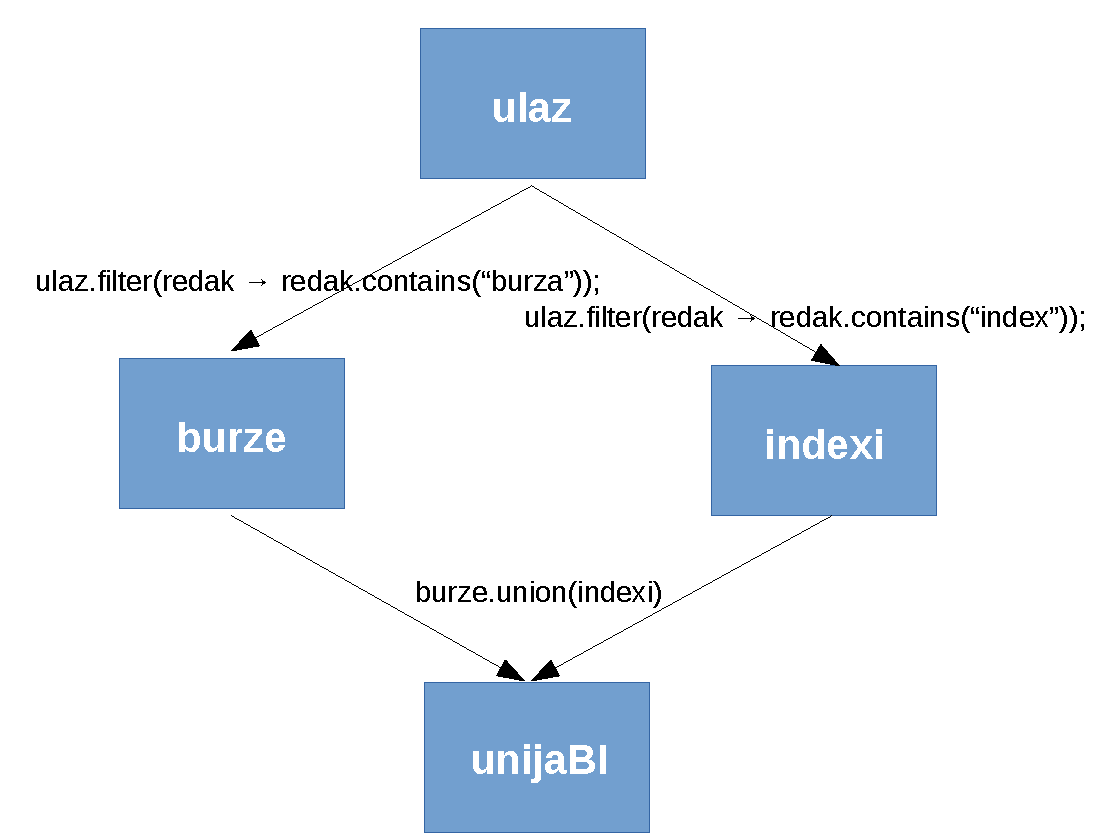
\includegraphics[scale = 0.8]{img/transformacijeCropped.pdf}
\caption{Transformacije nad skupovima podataka.}
\label{fig:burzeUnijaIndexiRDD}
\end{figure}

Tek prilikom poziva akcije \texttt{unijaBI.count()} se zapravo kreira  \texttt{ulaz}, na temelju njega \texttt{burza} i \texttt{indexi} i onda tek na temelju njih se kreira \texttt{unijaBI}. Iz  \texttt{unijaBI} ukupni broj linija dohvati se pozivom \texttt{unijaBI.count()}. 
Nakon što se to izračuna, svi skupovi podataka nestaju iz memorije.  Prilikom poziva akcije \texttt{unijaBI.first()} \textbf{ponovno} kreće obrada podataka gore navedenim redosljedom i sve ide iz početka.

Na prvi pogled ovo izgleda kao loša implementacija, ali budući da se ovdje radi o velikoj količini podataka i ne možemo ih nikako sve pohraniti u memoriju, ovo je zapravo logična implementacija. 
Ukoliko ne želimo svaki puta iz početka računati i kreirati \texttt{unijaBI}, trebamo ga pohraniti pozivom metode \texttt{persist()} i predavanjem odgovarajućeg parametra. Tablica \ref{tbl:razinePerzistencije} sadrži usporedbu različitih parametara koji se mogu predati metodi \texttt{persist()}.

\begin{table}[htb]
\scriptsize
\caption{Usporedba mogućih parametara za metodu \texttt{persist()}.}
\label{tbl:razinePerzistencije}
\centering
\begin{tabular}{lllll} 
\hline
Razina & Prostorno zauzeće & Procesorsko vrijeme & U memoriji & Na disku\\
\hline
\texttt{MEMORY\_ONLY} & Visoko & Nisko & Da & Ne  \\
\texttt{MEMORY\_ONLY\_SER} & Nisko & Visoko & Da & Ne  \\
\texttt{MEMORY\_AND\_DISK} & Visoko & Srednje & Dio & Dio \\
\texttt{MEMORY\_AND\_DISK\_SER} & Nisko & Visoko & Dio & Dio \\
\texttt{DISK\_ONLY} & Nisko & Visoko & Ne & Da \\
\hline
\end{tabular}
\end{table}

Iz tablice \ref{tbl:razinePerzistencije} očito je da postoje dvije osi usporedbe: spremanje na disk - spremanje u memoriju i spremanje u serijaliziranom obliku - spremanje u neserijaliziranom obliku. Postoji i parametar \texttt{MEMORY\_AND\_DISK} koji prvo podatke sprema u memoriju dok se memorija ne napuni, a kada se napuni, ostatak podataka se sprema na disk. Ono što razlikuje parametre koji sadrže sufiks \texttt{SER} i one koji ga ne sadrže je to što parametri sa sufiksom \texttt{SER} spremaju podatke u serijaliziranom obliku, a drugi ne.


\chapter{Napredno programiranje}
U ovom poglavlju opisane su neke napredne tehnike za rad s tehnologijom \emph{Apache Spark}. Objašnjen je algoritam \emph{PageRank}, a dana je i implementacija istog u primjeru \ref{lst:pagerank}.
\section{Primjer: Algoritam PageRank} \label{algoritamPageRank}
Zanimljivo je pitanje kako je \emph{Google} toliko dobar u rezultatima koje korisnik dobije na svoj upit, točnije, kako ispravno sortira po relevantnosti stranice od važnije prema manje važnoj? Odgovor na to daje algoritam \emph{PageRank} koji je dobio ime po jednom od osnivača \emph{Googlea}, Larry Pageu. Ovo potpoglavlje analizira upravo algoritam \emph{PageRank}. U nastavku je iznesena pojednostavljena verzija algoritma, a za više informacija moguće je konzultirati \cite{pageRank}.

\subsection{Upoznavanje s algoritmom}
Algoritam računa koliko je koja stranica važna po tome koliko drugih stranica upućuje na nju. Ideja je jednostavna: što više stranica ima poveznicu na neku stranicu \texttt{N}, to je stranica \texttt{N} važnija i time bolje rangirana. U obzir se uzima i koja stranica pokazuje na stranicu \texttt{N} (je li to stranica na koju sve ostale stranice pokazuju ili je to neka stranica na koju nitko ne pokazuje) kao i na koliko ostalih stranica ta stranica sadrži poveznice (nije isto ako je na cijeloj stranici samo jedna poveznica i ako na cijeloj stranici ima 1000 poveznica) i koliko su one same važne. Stranice na koje neka stranica \texttt{M} sadrži poveznice nazivamo \emph{susjedima} te stranice.
Pojednostavljena izvedba prikazana je u nastavku.

\newpage
\begin{enumerate}[label*=\arabic*.]
\item Početni rang svake stranice postavi se na $1.0$.
\item Ponavljaj \texttt{P} puta:
\begin{enumerate}[label*=\arabic*.]
\item Svaka stranica \texttt{\emph{n}} svim svojim susjedima šalje doprinos\\ \texttt{rang(\emph{n}) / brojSusjeda(\emph{n})}.
\item Postavi ukupni rang stranice prema formuli:\\ $0.15 + 0.85*\emph{ukupan primljeni doprinos}$.
\end{enumerate}
\end{enumerate}

Kako bi se što brže dobio što precizniji rezultat, važno je broj ponavljanja algoritma  \texttt{P} postaviti na prikladnu vrijednost. U praksi je dovoljno \texttt{P} postaviti na 10. 

Pretpostavimo raspored stranica kao na slici \ref{fig:pageRankSusjedi}.

\begin{figure}[htb]
\centering
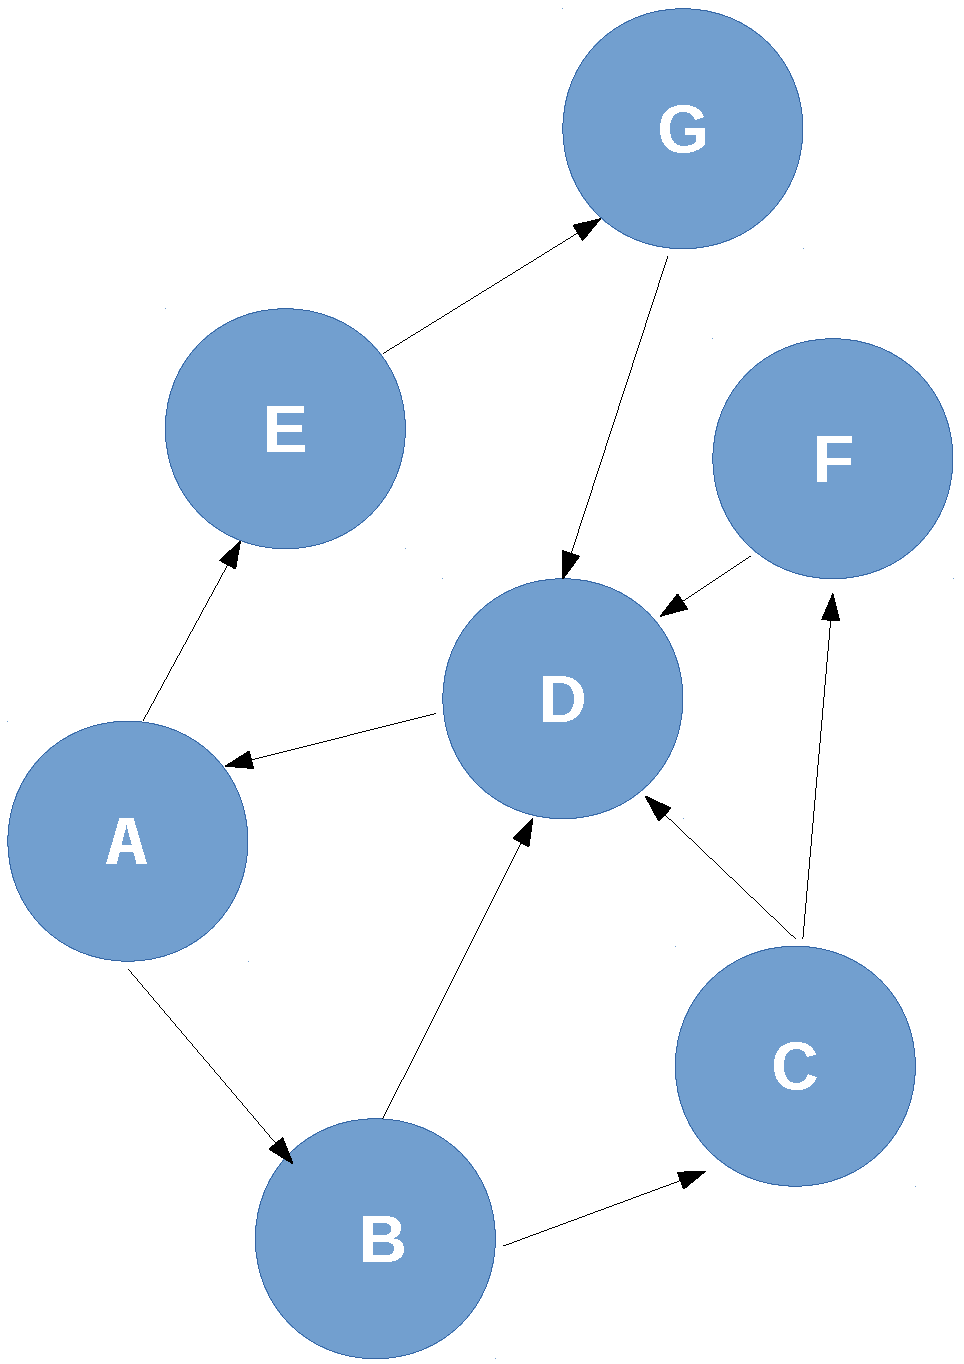
\includegraphics[scale = 0.5]{img/algoritamPageRankRucnoCropped.pdf}
\caption{Raspored susjeda u algoritmu}
\label{fig:pageRankSusjedi}
\end{figure}

U nastavku je raspisan algoritam \emph{PageRank} nad stranicama koje imaju susjede definirane kao na slici \ref{fig:pageRankSusjedi}. Ako stranica \texttt{N} sadrži poveznicu na stranicu \texttt{M} to je na toj istoj slici definirano tako da strelica počinje iz kruga s oznakom \texttt{N}, a vrh joj pokazuje na krug s oznakom \texttt{M}.

Intuitivno se čini da bi stranica \texttt{D} trebala biti najviše rangirana budući da najviše stranica upućuje na nju. Idemo to provjeriti. Za početak, odredimo susjede od svake stranice i postavimo rang svake stranice na $1.0$ kao što je prikazano u tablici \ref{tbl:pageRankKorak1}.

\begin{table}[htb]
\caption{Inicijalizacija rangova i određivanje susjeda}
\label{tbl:pageRankKorak1}
\centering
\begin{tabular}{lll} 
\hline
Stranica & Rang & Susjedi \\
\hline
A & $1.0$ & B, E\\
B & $1.0$ & C\\
C & $1.0$ & D, F\\
D & $1.0$ & A\\
E & $1.0$ & G\\
F & $1.0$ & D\\
G & $1.0$ & D\\
\hline
\end{tabular}
\end{table}

Sada se ponavljaju koraci 2.1 i 2.2 \texttt{P} puta. Ovdje je ponovljeno 2 puta i to bi trebalo biti dovoljno za razumjevanje algoritma.
Iz koraka 2.1 računa se doprinos koja šalje svaka od stranica. Doprinos stranice \texttt{A} koji ona šalje drugima iznosi $1.0 / 2 = 0.5$. Doprinos stranice \texttt{B} koji ona šalje drugima je $1.0 / 2 = 0.5$. Doprinos stranice \texttt{C} jednak je kao i doprinos stranica \texttt{A} i \texttt{B} jer imaju jednak rang i broj susjeda. Doprinos stranica \texttt{D}, \texttt{E}, \texttt{F} i \texttt{G} iznosi $1.0 / 1 = 1.0$. Rezultati za svaku od stranica prikazani su u tablici \ref{tbl:pageRankKorak21p1}.

\begin{table}[htb]
\caption{Izračun doprinosa koji šalje svaka od stranica.}
\label{tbl:pageRankKorak21p1}
\centering
\begin{tabular}{llll} 
\hline
Stranica & Rang & Susjedi & Doprinos drugima\\
\hline
A & $1.0$ & B, E & 0.5\\
B & $1.0$ & C, D & 0.5\\
C & $1.0$ & D, F & 0.5\\
D & $1.0$ & A & 1.0\\
E & $1.0$ & G & 1.0\\
F & $1.0$ & D & 1.0\\
G & $1.0$ & D & 1.0\\
\hline
\end{tabular}
\end{table}

Sada, za svaku od stranica se računa ukupna suma koju je ta stranica dobila od svojih susjeda po formuli danoj u koraku 2.2.
Budući da je stranica \texttt{A} susjed samo od stranice \texttt{D}, ukupni primljeni doprinos koji je primila stranica \texttt{A} je upravo doprinos koji stranica \texttt{D} može dati drugima, a to je $1.0$. Stranica \texttt{B} je susjed jedino stranici \texttt{A} i doprinos koji prima je upravo doprinos koji stranica \texttt{A} može u ovom trenutku dati drugima, a to je $0.5$. Stranica \texttt{C} je susjed jedino stranici \texttt{B} i zbog toga je njen ukupni primljeni doprinos $0.5$. Stranica \texttt{D} je susjed stranicama \texttt{B}, \texttt{C}, \texttt{F} i \texttt{G} pa je njen ukupni primljeni doprinos $0.5 + 0.5 + 1.0 + 1.0 = 3.0$. Ukupan primljeni doprinos za svaku od stranica nalazi se u tablici \ref{tbl:pageRankKorak22ap1}.

\begin{table}[htb]
\caption{Ukupni primljeni doprinos svake od stranica.}
\label{tbl:pageRankKorak22ap1}
\centering
\begin{tabular}{lllll} 
\hline
Stranica & Rang & Susjedi & Doprinos drugima & Ukupni primljeni doprinos\\
\hline
A & $1.0$ & B, E & 0.5 & 1.0\\
B & $1.0$ & C, D & 0.5 & 0.5\\
C & $1.0$ & D, F & 0.5 & 0.5\\
D & $1.0$ & A & 1.0 & 3.0\\
E & $1.0$ & G & 1.0 & 0.5\\
F & $1.0$ & D & 1.0 & 0.5\\
G & $1.0$ & D & 1.0 & 1.0\\
\hline
\end{tabular}
\end{table}

Nakon što je izračunat ukupni primljeni doprinos, vrijeme je za ponovni izračun ranga svake od stanica po formuli koja se nalazi u koraku 2.2. Novi rang stranice \texttt{A} iznosi $0.15 + 0.85 * 1.0 = 1.0$. Novi rang stanice \texttt{B} iznosi $0.15 + 0.85 * 0.5 = 0.575$. Novi rang stranice \texttt{C} iznosi isto $0.575$ jer stranica \texttt{C} i stranica \texttt{B} imaju jednaki ukupni primljeni doprinos. Novi rang stranice \texttt{D} je $0.15 + 0.85 * 3.0 = 2.7$. Nakon što se izračuna i postavi novi rang za svaku od stranica, nastupi situacija kao u tablici \ref{tbl:pageRankStanje1}

\begin{table}[htb]
\caption{Rang svake od stranica nakon prve iteracije.}
\label{tbl:pageRankStanje1}
\centering
\begin{tabular}{lll} 
\hline
Stranica & Rang & Susjedi \\
\hline
A & $1.0$ & B, E\\
B & $0.575$ & C, D\\
C & $0.575$ & D, F\\
D & $2.7$ & A\\
E & $0.575$ & G\\
F & $0.575$ & D\\
G & $1.0$ & D\\
\hline
\end{tabular}
\end{table}

Vidimo da je već u prvoj iteraciji algoritma stranica \texttt{D} iskočila sa svojim rangom od okoline. Ovo smo bili i pretpostavili budući da je stranica \texttt{D} susjed najvećem broju stranica, odnosno najveći broj stranica sadrži poveznicu na stranicu \texttt{D}. 

Idemo napraviti još jednu iteraciju i vidjeti što će se dogoditi s rangovima. 

Iz tablice \ref{tbl:pageRankStanje1} dohvaćamo rang i broj susjeda svake od stranica te računamo doprinos koji svaka od stranica može dati svojim susjedima prema već spomenutoj formuli u gornjem algoritmu u koraku 2.1. Doprinos koji stranica \texttt{A} šalje drugima iznosi $1.0 / 2 = 0.5$. Doprinos koji stranica \texttt{B} šalje je $0.575 / 2 = 0.2875$. Doprinos stranice \texttt{C} je jednak doprinosu stranice \texttt{B} budući da imaju jednak rang i broj susjeda. Doprinos stranice \texttt{D} iznosi $2.7 / 1 = 2.7$. Doprinos stranica \texttt{E} i \texttt{F} iznosi $0.575$, a doprinos stranice \texttt{G} je $1.0$. Rezultati izračuna koliko koja stranica doprinosi drugima prikazani su u tablici \ref{tbl:pageRankKorak21p2}.

\begin{table}[htb]
\caption{Izračun doprinosa koji šalje svaka od stranica u drugoj iteraciji.}
\label{tbl:pageRankKorak21p2}
\centering
\begin{tabular}{llll} 
\hline
Stranica & Rang & Susjedi & Doprinos drugima\\
\hline
A & $1.0$ & B, E & 0.5\\
B & $0.575$ & C, D & 0.2875\\
C & $0.575$ & D, F & 0.2875\\
D & $2.7$ & A & 2.7\\
E & $0.575$ & G & 0.575\\
F & $0.575$ & D & 0.575\\
G & $1.0$ & D & 1.0\\
\hline
\end{tabular}
\end{table}

Sada se ponovno računa ukupni primljeni doprinos svake od stranica. Tako za stranicu \texttt{A} se dobije da ukupni primljeni doprinos iznosi $2.7$ jer je ona jedino susjed stranici D. Ukupni primljeni doprinos stranice \texttt{B} je $0.5$ jer je upravo to iznos koliko stranica \texttt{A} doprinosi drugima, a stranica \texttt{B} je jedino susjed od stranice \texttt{A}. Stranica \texttt{C} ima ukupni primljeni doprinos $0.2875$ jer je upravo to iznos doprinosa stranice \texttt{B}, a stranica \texttt{C} je susjed jedino stranici \texttt{B}. Stranica \texttt{D} prima zbroj doprinosa svih stranica kojima je susjed odnosno zbroj doprinosa stranica \texttt{B}, \texttt{C}, \texttt{F} i \texttt{G}. Iz toga proizlazi da je ukupni primljeni doprinos stranice \texttt{D} $0.2875 + 0.2875 + 0.575 + 1.0 = 2.15$. Ukupni primljeni doprinos za svaku od stranica nalazi se u tablici \ref{tbl:pageRankKorak22ap2}.

\pagebreak

\begin{table}[htb]
\caption{Ukupni primljeni doprinos svake od stranica u drugoj iteraciji.}
\label{tbl:pageRankKorak22ap2}
\centering
\begin{tabular}{lllll} 
\hline
Stranica & Rang & Susjedi & Doprinos drugima & Ukupni primljeni doprinos\\
\hline
A & $1.0$ & B, E & 0.5 & 2.7\\
B & $0.575$ & C, D & 0.2875 & 0.5\\
C & $0.575$ & D, F & 0.2875 & 0.2875\\
D & $2.7$ & A & 2.7 & 2.15\\
E & $0.575$ & G & 0.575 & 0.5\\
F & $0.575$ & D & 0.575 & 0.2875\\
G & $1.0$ & D & 1.0 & 0.575\\
\hline
\end{tabular}
\end{table}

Nakon što je i u drugoj iteraciji izračunat ukupni primljeni doprinos, vrijeme je za ponovni izračun ranga svake od stanica po formuli koja se nalazi u koraku 2.2. Novi rang stranice \texttt{A} iznosi $0.15 + 0.85 * 2.7 = 2.445$. Novi rang stanice \texttt{B} iznosi $0.15 + 0.85 * 0.5 = 0.575$. Novi rang stranice \texttt{C} iznosi $0.15 + 0.85 * 0.2875 = 0.394375 $. Novi rang stranice \texttt{D} je $0.15 + 0.85 * 2.15 = 1.9775$.
Rang stranice \texttt{E} je $0.15 + 0.85 * 0.5 = 0.575$, a rang stranice \texttt{F} iznosi $0.15 + 0.85 * 0.2875 = 0.394375$. Konačno, rang stranice \texttt{G} je $0.15 + 0.85 * 0.575 = 0.63875$. Nakon što se postavi novi rang za svaku od stranica, nastupi situacija kao u tablici \ref{tbl:pageRankStanje2}

\begin{table}[htb]
\caption{Rang svake od stranica nakon druge iteracije.}
\label{tbl:pageRankStanje2}
\centering
\begin{tabular}{lll} 
\hline
Stranica & Rang & Susjedi \\
\hline
A & $2.445$ & B, E\\
B & $0.575$ & C, D\\
C & $0.394375$ & D, F\\
D & $1.9775$ & A\\
E & $0.575$ & G\\
F & $0.394375$ & D\\
G & $0.63875$ & D\\
\hline
\end{tabular}
\end{table}

Iz tablice \ref{tbl:pageRankStanje2} vidljivo je da je stranica \texttt{A} preuzela vodstvo. To se isto može intuitivno prihvatiti budući da skoro sve stranice pokazuju na stranicu \texttt{D}, a upravo \texttt{D} je jedina stranica koja pokazuje na \texttt{A}.

Nakon što se izvrti 10 iteracija, stvari se stabiliziraju. Graf koji opisuje kako se rangovi mijenjaju kroz 10 iteracija prikazan je slikom \ref{fig:grafRangIteracija}.

\begin{figure}[htb]
\centering
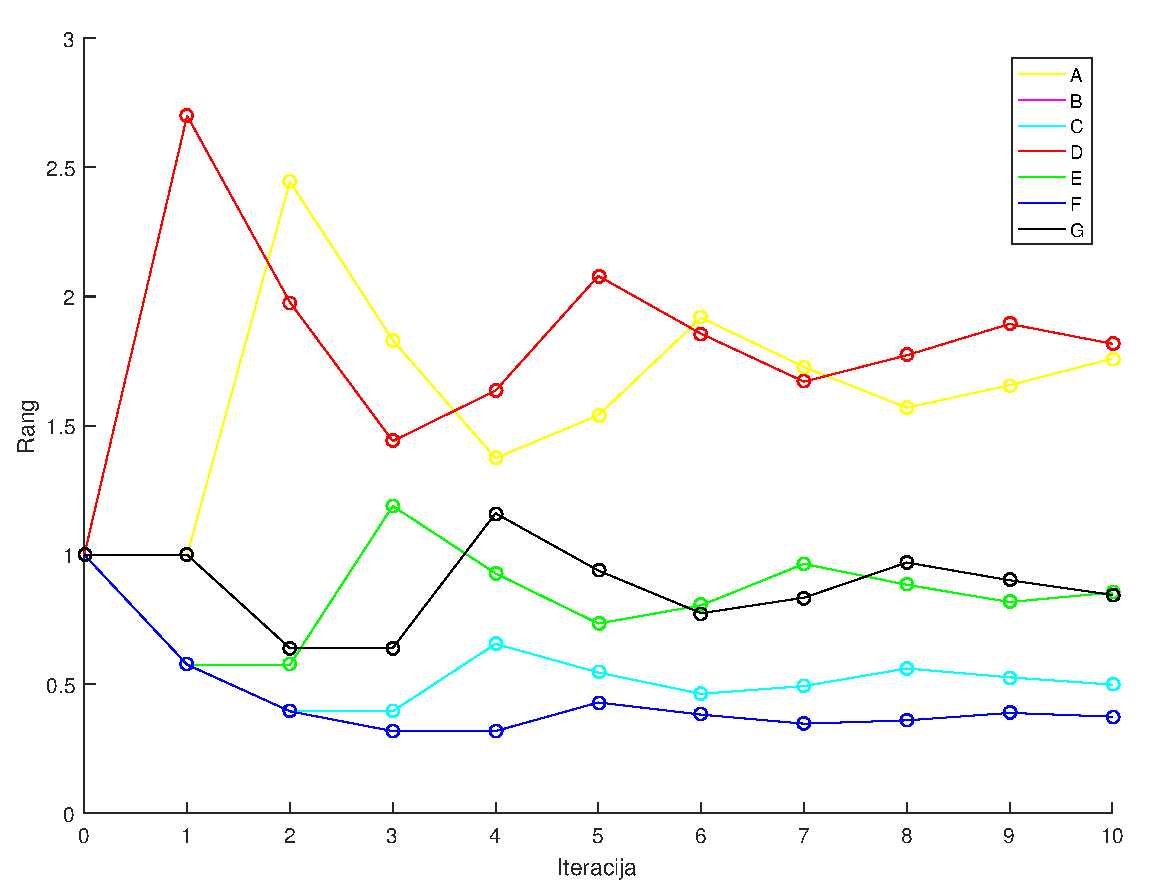
\includegraphics[scale = 0.5]{img/grafPageRankStraniceCropped.pdf}
\caption{Vrijednosti ranga ovisno o iteraciji}
\label{fig:grafRangIteracija}
\end{figure}

\subsection{Implementacija i analiza} \label{ssec:implAnalizaPRalg}
Kada je poznato kako "ručno" radi algoritam, ne bi trebao biti problem napisati programsku implementaciju koja se nalazi u primjeru \ref{lst:pagerank}. U ovom dijelu je osim samog koda napisana i detaljna analiza tog koda kako bi se dobilo što više informacija o tome kako radi tehnologija \emph{Apache Spark}. 

\vspace{5mm}
\begin{lstlisting}[numbers=left, label={lst:pagerank}, caption={Algoritam \emph{PageRank}.}, escapechar=|]
package hr.fer.zemris.naprednoProgramiranje;

import java.util.ArrayList;
import java.util.List;

import org.apache.spark.SparkConf;
import org.apache.spark.api.java.JavaPairRDD;
import org.apache.spark.api.java.JavaRDD;
import org.apache.spark.api.java.JavaSparkContext;

import com.google.common.collect.Iterables;

import scala.Tuple2;

/**
 * Program računa rang pojedine stranice. 
 * Očekuje se da svaki redak ulazne datoteke sadrži 
 * samo 2 stranice u formatu "StranicaA StranicaB", a taj
 * zapis predstavlja da je StranicaB susjed od StranicaA.
 * 
 * @author mmatak
 *
 */
public class AlgoritamPageRank {
	private static final String ULAZNA_DATOTEKA = "pageRankInput.txt";
	private static final int BROJ_ITERACIJA = 10;

	public static void main(String[] args) {
		// Inicijalizacija SparkContext-a.
		SparkConf conf = new SparkConf() |\label{line:initStart}|
				.setMaster("local") 
				.setAppName("Algoritam PageRank");
		JavaSparkContext sc = new JavaSparkContext(conf); |\label{line:initEnd}|

		// Učitavanje podataka.
		JavaRDD<String> ulaz = sc.textFile(ULAZNA_DATOTEKA); |\label{line:ucitavanje}|

		// Pročitaj sve ulazne URL-e i inicijaliziraj njihove susjede.
		JavaPairRDD<String, Iterable<String>> linkovi = ulaz.mapToPair(|\label{line:susjediInitStart}|
				redak -> {
					String[] elementi = redak.split("\\s+");
					return new Tuple2<String, String>(
						elementi[0],
						elementi[1]
						);
				}
			).distinct().groupByKey().cache(); |\label{line:susjediInitEnd}|
		// Svako ime susjeda zamijeni s 1.0 i vrati novi skup podataka.
		JavaPairRDD<String, Double> rangovi = linkovi.mapValues(value -> 1.0); |\label{line:initRangovi}|

		// iteracija 2. i 3. koraka algoritma
		for (int i = 0; i < BROJ_ITERACIJA; i++) { |\label{line:brIteracijaStart}|
			// za svaki link izracunaj njegovu doprinos drugim linkovima
			JavaPairRDD<String, Double> doprinosi =
			linkovi.join(rangovi).values().flatMapToPair(|\label{line:joinValues}|
				linkoviRang -> { 	|\label{line:linkoviRangPocetak}|
			
					int brojSusjeda = Iterables.size(linkoviRang._1); |\label{line:brojSusjeda}|
					List<Tuple2<String, Double>> rezultati = 
					new ArrayList<Tuple2<String, Double>>();
					
						for (String susjed : linkoviRang._1) { |\label{line:petljaStart}|
							rezultati.add(new Tuple2<String, Double>(
								susjed,
								linkoviRang._2 / brojSusjeda
								)
							);
						} |\label{line:petljaKraj}|
						
						return rezultati; |\label{line:linkoviRangKraj}|					
				}
			);
			rangovi = doprinosi
					.reduceByKey((v1, v2) -> v1 + v2) |\label{line:zbrojPoKljucu}|
					.mapValues(suma -> 0.15 + suma * 0.85); |\label{line:postaviRang}|
		} |\label{line:brIteracijaKraj}|
		// spremi u memoriju
		List<Tuple2<String, Double>> rangoviFinal = rangovi.collect(); |\label{line:spremanjePodataka}|
		// ispis
		for (Tuple2<String, Double> entry : rangoviFinal) {
			System.out.printf(
				"Stranica %s ima rang %.2f\n",
				 entry._1,
				 entry._2
			);
		}
		sc.close();
	}
}
\end{lstlisting}
\vspace{5mm}

Analizirajmo kod naveden u primjeru \ref{lst:pagerank}. 

Od linije \ref{line:initStart} do linije \ref{line:initEnd} inicijalizira se glavno računalo i ime aplikacije. Ovdje je glavno računalo postavljeno na \texttt{local} budući da se aplikacija odvija na lokalnom računalu, a ne na grozdu. Ključna riječ koja se preda metodi \texttt{setMaster()} predstavlja URL glavnog računala u grozdu. Za lokalni rad, dovoljno je napisati \texttt{local}, ali mogući oblici su i \texttt{local[N]} te \texttt{local[*]}. Ovdje \texttt{N} predstavlja željeni broj dretvi, a \texttt{*} traži da se vrti onoliko dretvi koliko ima procesorskih jezgri. Ukoliko se izvršava rad na grozdu, potrebno je predati drukčiji argument\footnote{Ovisno o vrsti grozda, ide različit argument. Više informacija moguće je pronaći na \url{http://spark.apache.org/docs/latest/submitting-applications.html#master-urls}}. Ime aplikacije postavljeno je na temelju algoritma kojeg aplikacija implementira.

Linija \ref{line:ucitavanje} obavlja inicijalizaciju \emph{otpornog raspodijeljenog skupa podataka} čitajući podatke iz datoteke čija je putanja zadana varijablom \texttt{ULAZNA\_DATOTEKA}.

Od linije \ref{line:susjediInitStart} do linije \ref{line:susjediInitEnd} obavlja se pridruživanje susjeda svakoj stranici. Svaki se redak iz skupa \texttt{ulaz} podijeli na dva elementa - element prije i element poslije razmaka. Ta dva elementa predstavljaju uređeni par (\emph{ključ}, \emph{vrijednost}) gdje je stranica koja je prije razmaka \emph{ključ}, a stranica nakon razmaka \emph{vrijednost}. To znači da je stranica \emph{vrijednost} susjed od stranice \emph{ključ}. Budući da su dozvoljeni duplikati u ulaznom skupu podataka tj. mogu postojati dva identična retka koja govore kako stranica \emph{N} ima susjeda \emph{M}, to se mora uzeti u obzir. Za rangiranje stranice nije bitno koliko poveznica stranica \emph{N} sadrži na stranicu \emph{M}. U ovoj implementaciji, svejedno je radi li se o 1 ili 1000 poveznica jer su to sve iste poveznice. Da bi se osiguralo da ne postoji niti jedan duplikat, poziva se metoda \texttt{distinct()}.

Pozivom metode \texttt{groupByKey()} obavlja se \emph{spajanje} uređenih parova s istim ključem, a njihove vrijednosti spremamo u listu. Primjerice, postoji li kolekcija uređenih parova (\emph{A}, \emph{B}), (\emph{A}, \emph{C}), (\emph{A}, \emph{D}) i ako se nad tom kolekcijom pozove se \texttt{groupByKey()} rezultat će biti novi skup podataka predstavljen uređenim parom (\emph{A}, \{\emph{B}, \emph{C}, \emph{D}\}). \emph{Vrijednost} tog uređenog para je iterabilna (implementira sučelje \texttt{Iterable}) i zbog toga je povratna vrijednost u obliku \texttt{JavaPairRDD<String, Iterable<String>{}>}. Rezultat je skup podataka \texttt{linkovi} predstavljen uređenim parovima gdje su \emph{ključevi} stranice, a \emph{vrijednosti} susjedi tih stranica. Konačno, kako se ne bi ovo moralo svaki puta ispočetka računati, rezultat se pohranjuje u memoriju pozivom metode \texttt{cache()}. Poziv metode \texttt{cache()} ima isti učinak kao i da se pozove metoda \texttt{persist()} s argumentom \texttt{MEMORY\_ONLY}.

Linija \ref{line:initRangovi} iz skupa podataka \texttt{linkovi} "provuče" svaku od \emph{vrijednosti} (čitava kolekcija je zapravo jedna \emph{vrijednost}) kroz funkciju koja tu čitavu kolekciju samo preslika u \emph{vrijednost} $1.0$. Sada je nastao novi skup uređenih parova koji za \emph{ključ} imaju stranicu, a za \emph{vrijednost} $1.0$. Ovim postupkom je zapravo postavljen rang svake stranice na početnu vrijednost.

Poziv naredbe \texttt{linkovi.join(rangovi)} u liniji \ref{line:joinValues} vraća novi skup podataka koji kao \emph{ključeve} ima \emph{ključeve} iz skupova \texttt{linkovi} i \texttt{rangovi} (bez dupliciranja), a odgovarajuće \emph{vrijednosti} su uređeni parovi \emph{vrijednosti} iz tih skupova. Preciznije rečeno, \texttt{join(\emph{drugiSkupPodataka})} ako je pozvan nad skupovima uređenih parova oblika (\emph{K},\emph{V}) i (\emph{K}, \emph{W}) kao rezultat vraća skup podataka uređenih parova oblika (\emph{K},(\emph{V}, \emph{W})). Ukoliko postoje različiti \emph{ključevi} u skupovima podataka nad kojima se izvršava \texttt{join()}, parovi s stim \emph{ključem} su ignorirani. Jedino se "uparuju" uređeni parovi s istim \emph{ključem}. Metoda \texttt{values()} vraća skup svih \emph{vrijednosti} iz skupa podataka dobivenog pozivom metode \texttt{join()}. U ovom primjeru metoda \texttt{values()} vraća skup uređenih parova gdje je \emph{ključ} kolekcija susjeda neke stranice, a \emph{vrijednost} rang te stranice. Metoda \texttt{flatMapToPair()} kao argument prima funkciju koja implementira sučelje \texttt{PairFlatMapFunction<T,K2,V2>}. Ta funkcija prima element tipa \texttt{T} i vraća nula ili više uređenih parova oblika (\texttt{K2}, \texttt{V2}). Metoda \texttt{flatMapToPair()} zapravo "provuče" svaki element skupa nad kojim je pozvana kroz funkciju koju primi kao argument i na kraju, na temelju uređenih parova koje je ta funkcija vratila, kreira skup podataka oblika (\texttt{K2}, \texttt{V2}). Element koji se "provlači" imenovan je varijablom \texttt{linkoviRang}.

Od linije \ref{line:linkoviRangPocetak} do linije \ref{line:linkoviRangKraj} obrađuju se podatci koji su predstavljeni uređenim parovima oblika (\emph{ključ}, \emph{vrijednost}) gdje je \emph{ključ} kolekcija susjeda neke stranice, a \emph{vrijednost} rang te stranice.

Linija \ref{line:brojSusjeda} zapravo dohvaća veličinu kolekcije koja je predstavljena \emph{ključem}, odnosno varijablu \texttt{brojSusjeda} postavlja na onu vrijednost koliko stranica koja se trenutno obrađuje ima susjeda. 

Od linije \ref{line:petljaStart} do linije \ref{line:petljaKraj} proteže se petlja koja u listu \texttt{rezultati} sprema uređene parove oblika (\emph{ključ}, \emph{vrijednost}) gdje je \emph{ključ} susjed, a \emph{vrijednost} doprinos tom susjedu stranice koja se trenutno obrađuje. 

Funkcija \texttt{flatMapToPair()} spaja sve vraćene rezultate u jedan skup i  sada se u skupu podataka \texttt{doprinosi} nalaze uređeni parovi gdje je \emph{ključ} stranica, a \emph{vrijednost} doprinos neke stranice toj stranici. Budući da neka stranica ne mora biti susjed samo jednoj stranici, u tom skupu podataka se može naći više parova s istim ključem - svaka vrijednost je doprinos od neke druge stranice. 

Linija \ref{line:zbrojPoKljucu} "spaja" sve parove s istim \emph{ključem} tako što od više uređenih parova s istim \emph{ključem} stvori jedan uređeni par s tim \emph{ključem}, a \emph{vrijednosti} zbroji. Time je zapravo izračunat ukupni primljeni doprinos svake od stranica i nastao je novi skup uređenih parova oblika (\emph{stranica}, \emph{ukupni primljeni doprinos}). 

Linija \ref{line:postaviRang} dohvaća \emph{vrijednosti} iz tih uređenih parova i na temelju njih računa nove \emph{vrijednosti} i postavlja ih kao trenutne \emph{vrijednosti}. Nove \emph{vrijednosti} su zapravo novi rangovi svake od stranica. Sada se u varijabi \texttt{rangovi} nalaze uređeni parovi (\emph{stranica}, \emph{rang}) . 

Postupak od linije \ref{line:brIteracijaStart} do linije \ref{line:brIteracijaKraj} ponavljamo potrebni broj puta kako bi se rang svake od stanica postavio na što ispravniju vrijednost. Kao što je već rečeno, u praksi je to desetak puta pa je tako i u ovom primjeru.

Kada su izračunati rangovi svake od stanica, sve što još treba je ispisati podatke. Kako bi se uštedilo na vremenu (ponovno računanje rangova svaki puta kada treba raditi nešto s tim rangovima), dohvaćamo sve podatke iz skupa podataka \texttt{rezultati} i spremamo ih u varijablu \texttt{rezultatiFinal}. Taj dio je prikazan linijom \ref{line:spremanjePodataka}.

Konačno, u \texttt{for} petlji iteriramo po elementima liste \texttt{rezultatiFinal} te ispišemo ime i rang stranice. Na kraju zatvorimo \emph{SparkContext}.


\section{Skupovi podataka kao uređeni parovi}
U primjeru \ref{lst:pagerank} već je uveden pojam skupa podataka koji je predstavljen uređenim parom (\emph{ključ}, \emph{vrijednost}). U ovoj tehnologiji takav skup podataka nije rijetkost i zbog toga postoji niz transformacija nad upravo tim oblikom skupa podataka, a neke od njih su već objašnjene u potpoglavlju \ref{ssec:implAnalizaPRalg}. Osnovne informacije mogu se pronaći u tablicama \ref{tbl:transformacijeJedanPairRDD} i \ref{tbl:transformacijeDvaPairRDD}, a za više informacija, konzultirati službenu dokumentaciju \cite{officialDocumentation}.

\begin{table}[htb]
\caption{Neke od transformacija nad jednim skupom podataka koji je predstavljen uređenim parovima. Primjer: \{(1, 2), (3, 4), (3, 6)\}.}
\label{tbl:transformacijeJedanPairRDD}
\centering
\begin{tabular}{lp{10cm}} 
\hline
Transformacija & Opis\\
\hline

\texttt{reduceByKey(\emph{func})} & Kombinira vrijednosti s istim \emph{ključem}. Primjer korištenja je  \texttt{rdd.reduceByKey((x,y) -> x + y)}, a rezultat je onda \{(1, 2), (3, 10)\}.\\

\texttt{groupByKey()} & Grupira vrijednosti s istim \emph{ključem}.\newline Primjer korištenja je \texttt{rdd.groupByKey()}, a rezultat je  \{(1, [2]), (3, [4, 6])\}.\\

\texttt{mapValues(\emph{func})} & Primjena funkcije nad svakom \emph{vrijednosti} u uređenom paru, \emph{ključ} ostaje nepromijenjen. Primjer korištenja je \texttt{rdd.mapValues(x -> x + 10)}, a rezultat izvođenja je \{(1, 12), (3, 14), (3, 16)\}.\\

\texttt{keys()} & Vraća novi skup podataka koji se sastoji od svih \emph{ključeva}. Primjer korištenja je \texttt{rdd.keys()}, a rezultat je \{1, 3, 3\}.\\

\texttt{values()} & Vraća novi skup podataka koji se sastoji od svih \emph{vrijednosti}. Primjer korištenja je \texttt{rdd.values()}, a rezultat je \{2, 4, 6\}.\\
\hline
\end{tabular}
\end{table}

Često postoji potreba za transformacijom koja je kombinacija dva skupa podataka. Primjerice, spajanje tablica iz baze podataka. Te stvari su moguće i ovdje, a samo neke od transformacija prikazane su u tablici \ref{tbl:transformacijeDvaPairRDD}. Osim transformacija, postoje i akcije koje je moguće izvoditi nad otpornim raspodijeljenim skupom podataka koji je predstavljen kao uređeni par, ali radi formata ovog rada, nije napisana još jedna tablica gdje bi te akcije bile objašnjene. Za informacije o akcijama konzultirati \cite{officialDocumentation}.

\begin{table}[htb]
\caption{Neke od transformacija nad dva skupa podataka koji su predstavljeni uređenim parovima. Primjer: rdd = {(1, 2), (3, 4), (3, 6)}, drugi = {(3,9)}.}
\label{tbl:transformacijeDvaPairRDD}
\centering
\begin{tabular}{lp{10cm}} 
\hline
Transformacija & Opis \\
\hline

\texttt{subtractByKey} & Briše parove koji imaju iste \emph{ključeve}. \newline Primjer korištenja je \texttt{rdd.subtractByKey(drugi)}, a odgovarajući rezultat je \{(1, 2)\}.\\

\texttt{join} & Obavlja operaciju \emph{prirodnog spajanja} \engl{inner join}. Primjer korištenja je \texttt{rdd.join(drugi)}, a odgovarajući rezultat je \{(3, (4, 9)), (3, (6, 9))\}.\\
\hline
\end{tabular}
\end{table}

Ono što je još često potrebno, a nije već spomenuto jest sortiranje podataka.\\ Tehnologija \emph{Apache Spark} omogućuje i sortiranje uređenih parova po \emph{ključu}. Transformacija se naziva \texttt{sortByKey} i primjer poziva je \texttt{rdd.sortByKey()}. Prima argument treba li sortirati uzlazno (podrazumijevana vrijednost) ili silazno. Dodatno, moguće je i predati komparator koji će usporediti ključeve. 

\section{Čitanje i spremanje podataka }
U ranijim primjerima prikazano je kako ostvariti čitanje podataka iz tekstualne datoteke kao i kako zapisati rezultat u neku tekstualnu datoteku. Neki od podržanih oblika tekstualnih datoteka su JSON, CSV i TSV. Tehnologija \emph{Apache Spark} omogućuje i puno više. Između ostalog, moguće je čitati i pisati direktno u bazu podataka (Cassandra, HBase, Elasticsearch, JDBC), koristiti  strukturirane izvore uključujući JSON i Apache Hive, a isto tako moguće je čitati i podatke koji su spremljeni na raspodijeljenom sustavu datoteka poput NFS, HDFS ili Amazon S3.

Datoteke u JSON obliku se učitaju poput tekstualne datoteke, a zatim se parsira prema formatu JSON. Za parsiranje ovog formata se u pravilu koriste gotove biblioteke, a popularna biblioteka za Javu naziva se \emph{Jackson}. Više informacija o tim bibliotekama može se pronaći na poveznici \footnote{\url{http://geokoder.com/java-json-libraries-comparison}}. 

Više informacija o čitanju i spremanju podataka potražiti u poglavlju \emph{Loading and saving your data} \cite{learningSpark}.

\section{Dijeljene varijable}
Funkcija koju predamo metodi \texttt{map()} vidi varijable koje su definirane u \emph{pozivajućem programu}, ali svaki \emph{zadatak} \engl{task} koji se vrti na \emph{grozdu} dobije svoju kopiju vrijednosti tih varijabli, a nove vrijednosti tih varijabli nisu propagirane \emph{pozivajućem programu}. Riješenje ovog problema su dijeljene varijable \engl{shared variables}. Ime su dobile po tome što je njihova \emph{ispravna} vrijednost vidljiva svuda u grozdu.

\subsection{Odašiljatelji}
Ukoliko je potrebno dohvaćati vrijednost neke varijable na cijelom grozdu, potrebna je \emph{varijabla odašiljatelj} \engl{broadcast variable}. Ta varijabla se pohranjuje u memoriji i zbog toga ne smije zauzimati puno prostora. Također, takva varijabla je nepromjenjiva \engl{immutable}. Moguće je slati i promjenjivu varijablu, ali ta promjena će biti jedino vidljiva na tom čvoru koji je promjenu napravio, a takvo ponašanje u pravilu nije poželjno. 

Kao što je navedeno u \cite{officialDocumentation}, \emph{odašiljatelji} se mogu koristiti kao nepromjenjive pregledne tablice \engl{lookup table}. 
Pretpostavimo da radimo na aplikaciji koja u bazi ima dvije tablice, tablicu koja pamti identifikator i ime naselja te tablicu koja pamti identifikator korisnika koji se prijavio i identifikator naselja gdje se prijavio. Primjer takvih tablica su tablice \ref{tbl:naselja} i \ref{tbl:prijave}.

\begin{table}[htb]
\caption{Tablica \texttt{naselja}.}
\label{tbl:naselja}
\centering
\begin{tabular}{ll} 
\hline
\texttt{id} & \texttt{ime}\\
\hline
1 & Centar\\
2 & Maksimir\\
3 & Jordanovac\\
4 & Siget\\
5 & Dubrava\\
\hline
\end{tabular}
\end{table}

U tablici \ref{tbl:naselja} nalaze se imena naselja s odgovarajućim identifikacijskim brojevima, a u tablici \ref{tbl:prijave} nalaze se prijave korisnika i identifikator odgovarajućeg naselja gdje je prijava zaprimljena.

\begin{table}[htb]
\caption{Tablica \texttt{prijave}.}
\label{tbl:prijave}
\centering
\begin{tabular}{ll} 
\hline
\texttt{id\_korisnik} & \texttt{id\_naselje}\\
\hline
112312 & 1\\
243242 & 2\\
254331 & 2\\
432115 & 1\\
567893 & 4\\
537893 & 4\\
\hline
\end{tabular}
\end{table}

Zadatak je saznati ime naselje za svaku od prijava. Pretpostavka je da postoji jako puno prijava, a ne previše naselja tj. prijave su u nekoj velikoj tablici, a naselja su u maloj tablici. Pri obavljanju klasične transformacije \texttt{join}, podatci obje tablice bi putovali svuda po mreži i to bi uzelo puno vremena i mrežnih resursa. Ukoliko je potrebno napraviti \texttt{join} male i velike tablice, bolje rješenje je malu tablicu (koja stane u memoriju i ne mijenja se) postaviti kao varijablu \emph{odašiljatelj}. Na taj način, jedino će mala tablica putovati preko mreže. U ovom primjeru, mala tablica je tablica  \ref{tbl:naselja} (\texttt{naselja}), a velika tablica je tablica \ref{tbl:prijave} (\texttt{prijave}). 

Varijable koje su postavljene kao \emph{odašiljatelj} preko mreže se prenose protokolom \emph{bittorrent}. To znači da što više čvorova treba tu varijablu, ta varijabla se brže širi po mreži\footnote{Više informacija o bittorent protokolu na stranici \url{http://www.bittorrent.org/}}. 

\vspace{5mm}
\begin{lstlisting}[numbers=left, label={lst:odasiljateljPrimjer}, caption={Korištenje odašiljatelja.}, escapechar=|]
package hr.fer.zemris.naprednoProgramiranje;

import java.util.Map;

import org.apache.spark.SparkConf;
import org.apache.spark.api.java.JavaPairRDD;
import org.apache.spark.api.java.JavaSparkContext;
import org.apache.spark.broadcast.Broadcast;

import scala.Tuple2;

public class Primjer5 {
	public static void main(String[] args) {
		// Inicijalizacija SparkContext-a.
		SparkConf conf = new SparkConf()
				.setMaster("local")
				.setAppName("Razasiljane varijable");
				
		try (JavaSparkContext sc = new JavaSparkContext(conf)) {
		
			// inicijalizacija naselja
			JavaPairRDD<String, String> naseljaRDD = sc
				.textFile("tblNaselja.txt")
				.mapToPair(
					redakTablice -> {
						String[] redak = redakTablice.split(",");
						return new Tuple2<String, String>(
							redak[0], redak[1]
							);
					}
				);
					
			// prijave
			JavaPairRDD<String, String> prijaveRDD = sc
					.textFile("tblPrijave.txt")
					.mapToPair(redakTablice -> {
						String[] redak = redakTablice.split(",");
						return new Tuple2<String, String>(
							redak[0], redak[1]
							);
						}
					);
							
			// odasiljanje read only varijable "naselja" kroz grozd
			final Broadcast<Map<String, String>> naselja = 
				sc.broadcast(naseljaRDD.collectAsMap());

			
			JavaPairRDD<String, Tuple2<String, String>> imenovanePrijave = prijaveRDD
					.mapToPair(
						prijava -> new Tuple2<String, Tuple2<String, String>>(
								prijava._1,
								new Tuple2<String, String>(
									prijava._2,
									naselja.getValue().get(prijava._2)
								)
							)
						);
			//ispis
			for (Tuple2<String, Tuple2<String, String>> element :
			 	imenovanePrijave.collect()) {
				System.out.printf(
					"Id prijave: %s \t Ime naselja: %s\n",
						element._1,
						element._2._2
					);
			}
		}
	}
}
\end{lstlisting}
\vspace{5mm}

U primjeru \ref{lst:odasiljateljPrimjer} pokazano je korištenje odašiljatelja. Osim toga, u tom primjeru je \emph{SparkContext} inicijaliziran u \emph{try-catch} bloku naredbi. Budući da \emph{SparkContext} implementira sučelje \texttt{Closeable}, to je garancija da ako ga otvorimo \emph{try-catch} inicijalizacijskom bloku da će biti i pravovremeno zatvoren.

Program čita iz datoteke \texttt{tblNaselja.txt} podatke o naseljima koji su zapisani u obliku \emph{id\_naselja, ime\_naselja}. Podatci o prijavama imaju oblik \emph{id\_prijave, id\_naselja} i čitaju se iz datoteke \texttt{tblPrijave.txt}. Podatci u tim datotekama jednaki su podatcima iz tablica \ref{tbl:naselja} i \ref{tbl:prijave}. Nakon što su podatci učitani, kreirani su skupovi podataka. Zatim se skup podataka koji predstavlja tablicu \ref{tbl:naselja} pretvorio u mapu gdje je \emph{ključ} identifikator naselja, a \emph{vrijednost} ime naselja. Takva mapa je \emph{odaslana} svuda po mreži. 

Nakon toga, za svaku prijavu, kreiran je novi uređeni par koji za \emph{ključ} ima identifikator prijave, a za vrijednost objekt \texttt{Tuple2} koji za prvu vrijednost ima identifikator nasilja, a za drugu vrijednost ime tog naselja. Razred \texttt{Tuple2} preuzet je iz programskog jezika Scala i predstavlja uređeni par (\emph{vrijednost\_1}, \emph{vrijednost\_2}). Shodno tome, prvoj vrijednosti se pristupa preko \texttt{element.\_1}, a drugoj vrijednost preko \texttt{element.\_2}.

Na kraju su ispisani svi dobiveni podatci, a rezultat je prikazan u primjeru \ref{lst:rezultati}.
\begin{lstlisting}[label={lst:rezultati}, caption={Identifikatori prijave i imena naselja odakle su prijave poslane.}]
Id prijave: 112312 	 Ime naselja: Centar
Id prijave: 243242 	 Ime naselja: Maksimir
Id prijave: 254331 	 Ime naselja: Maksimir
Id prijave: 432115 	 Ime naselja: Centar
Id prijave: 567893 	 Ime naselja: Siget
Id prijave: 537893 	 Ime naselja: Siget
\end{lstlisting}

\subsection{Akumulatori}
Ako se odašiljatelje gleda kao globalne \emph{gettere}, \emph{akumulatore} \engl{accumulators} se može gledati kao na globalne \emph{settere}. Za razliku od odašiljatelja koji svim čvorovima dojavljuju vrijednost, akumulatori akumuliraju, odnosno dohvaćaju vrijednost svakog čvora. Ideja je jednostavna, ako je potrebno s više radnih čvorova mijenjati nekakvu globalnu varijablu, ta varijabla se postavi kao akumulator.

U datoteci \texttt{log.txt} pohranjeni su zapisi pristupanju na poslužitelj. Svaki zapis je u novom retku. Ukoliko u nekom retku postoji riječ \texttt{error}, taj zapis nije valjan. Svaki drugi zapis je valjan. Zadatak je izbrojati koliko postoji valjanih zapisa i koliko postoji zapisa koji nisu valjani. Jedno od riješenja je koristiti dva akumulatora: jedan za valjane zapise i drugi za zapise koji nisu valjani. Programska implementacija tog rješenja dana je u primjeru \ref{lst:akumulatoriPrimjer}.

\vspace{5mm}
\begin{lstlisting}[numbers=left, label={lst:akumulatoriPrimjer}, caption={Korištenje akumulatora.}, escapechar=|]
package hr.fer.zemris.naprednoProgramiranje;

import org.apache.spark.Accumulator;
import org.apache.spark.SparkConf;
import org.apache.spark.api.java.JavaRDD;
import org.apache.spark.api.java.JavaSparkContext;

public class Primjer6 {
	public static void main(String[] args) {
		SparkConf conf = new SparkConf()
				.setMaster("local")
				.setAppName("Koristenje akumulatora");
		try (JavaSparkContext sc = new JavaSparkContext(conf)) {
			// inicijalizacija naselja
			JavaRDD<String> zapisi = sc.textFile("log.txt");

			// inicijalizacija akumulatora
			Accumulator<Integer> valjaniZapisi = sc.accumulator(0);
			Accumulator<Integer> neValjaniZapisi = sc.accumulator(0);

			// obrada podataka
			for (String redak : zapisi.collect()) {
				if (redak.contains("error")) {
					neValjaniZapisi.add(1);
				} else {
					valjaniZapisi.add(1);
				}
			}
			// ispis rezultata
			System.out.printf("Valjanih zapisa ima %d\n",
					valjaniZapisi.value());
			System.out.printf("Nevaljanih zapisa ima %d\n",
					neValjaniZapisi.value());
		}
	}
}
\end{lstlisting}

Primjer \ref{lst:akumulatoriPrimjer} učita novi skup podataka, inicijalizira akumulatore te za svaki redak, ovisno sadrži li redak riječ \emph{error} ili ne, poveća vrijednost odgovarajućeg akumulatora.

U primjeru \ref{lst:akumulatoriPrimjer} korišteni su cjelobrojni akumulatori. Osim \emph{Integer} tipa podataka, postoje akumulatori i za \emph{Long}, \emph{Double} te \emph{Float} tip podataka. Ukoliko je potrebno, moguće je kreirati i akumulator za svoj vlastiti tip podataka. Više informacija o akumulatorima moguće je pronaći u \cite{workingSets}.
\chapter{Zaključak} 
Danas već postoji više podataka u digitalnom obliku nego ikada prije. U budućnosti se pretpostavlja da će ih biti još i više. Tehnologija \emph{Apache Spark} nudi mogućnost obrade velikog skupa podataka. U radu je pokazano da ima bogato programsko sučelje za programski jezik Java i da se u svega nekoliko naredbi može dosta dobro obraditi te podatke. 

Kao nastavak ovog rada predlaže se istražiti kako instalirati i koristiti ovu tehnologiju na grozdu. Također bi bilo dobro i detaljnije istražiti te opisati svaki od gradivnih elemenata od kojih se ova tehnologija sastoji. Ovo je tehnologija koja je svakim danom sve popularnija i u budućnosti bi mogla imati široku primjenu.

\begin{thebibliography}{9}
\bibitem{officialDocumentation}
  Službena dokumentacija projekta \emph{Apache Spark} \url{http://spark.apache.org/docs/latest/}, posjećeno 1.5.2016
\bibitem{learningSpark}
  Holden Karau, Andy Konwinski, Patrick Wendell i Matei Zaharia
  \emph{Learning Spark, lighting-fast}, O'Reilly 2015.
\bibitem{marcupic}
  Marko Čupić,
  \emph{Programiranje u Javi},
  verzija 0.3.26
  URL: \url{http://java.zemris.fer.hr/nastava/opjj/book-2015-09-30.pdf}
\bibitem{workingSets}
  ZAHARIA, Matei, et al. Spark: Cluster Computing with Working Sets. \emph{HotCloud 10}, 2010, 10: 10-10.
\bibitem{pageRank}
	XING, Wenpu; GHORBANI, Ali. Weighted pagerank algorithm. In: \emph{Communication Networks and Services Research, 2004. Proceedings. Second Annual Conference on.} IEEE, 2004. p. 305-314
\end{thebibliography}

\newpage
% Dodatak nije obavezan
\begin{appendices}
\chapter{Instalacija}
\label{ch:instalacijaSpark}
Ovdje je prikazana instalacija na operacijskom sustavu \emph{Ubuntu 15.10}. Ovo nije veliko ograničenje jer se iz ovih uputa može zaključiti i kako instalacija ide za neki drugi operacijski sustav.

Za početak je potrebno imati instaliranu Javu, a je li Java instalirana na računalu se može provjeriti tako što se u naredbenom retku unese sljedeća naredba:\\
\texttt{java -version}. Kao rezultat se dobije trenutno instalirana verzija Jave. Ukoliko Java nije instalirana, potrebno ju je najprije instalirati (ili ispravno podesiti okruženje varijable \texttt{PATH}). Više informacija o instalaciji se može pronaći u \cite{marcupic}.

Jednom kada je Java instalirana, sve što treba napraviti je otići na službene stranice: \url{https://spark.apache.org/downloads.html}, odabrati najnoviju verziju (aa vrijeme pisanja ovog rada to je verzija \emph{1.6.1 Mar 09 2016}), izabrati odgovarajući paket te pokrenuti dohvaćanje odgovarajuće \emph{.tgz} arhive. Najjednostavnije je odabrati neki \emph{pre-built} paket, primjerice \emph{Pre-built for Hadoop 2.6 and later}. Daljnji koraci instalacije su napisani pod pretpostavkom da je dohvaćena ta verzija paketa. Moguće je instalirati i \emph{Source code} varijantu paketa, ali taj postupak instalacije ovdje nije opisan. 

Nakon što je dohvaćena odgovarajuća arhivu, potrebno ju je raspakirati.\\ Raspakiranje arhive moguće je napraviti preko naredbe:
\begin{lstlisting}[language=bash]
$ tar -xvf spark-1.6.1-bin-hadoop2.6.tgz
\end{lstlisting}
Nakon toga, dobra je praksa premjestiti instalaciju u neki prikladniji direktorij. Tako nešto može se napraviti na sljedeći način:
\begin{lstlisting}[language=bash]
$ mv Downloads/spark-1.6.1-bin-hadoop2.6 faks/spark/
\end{lstlisting}
Ovim korakom je instalacija završena. 

Kako bi bili sigurni da je instalacija uspješna, potrebno je pozicionirati se u \emph{bin} direktorij te u terminalu upisati \texttt{./spark-shell}. Ispis bi trebao biti sličan ovome:

\begin{lstlisting}[language=bash]
mmatak@martins-beast:~/faks/spark/bin$ ./spark-shell
Welcome to
      ____              __
     / __/__  ___ _____/ /__
    _\ \/ _ \/ _ `/ __/  '_/
   /___/ .__/\_,_/_/ /_/\_\   version 1.6.1
      /_/

Using Scala version 2.10.5 (OpenJDK 64-Bit Server VM, Java 1.8.0_91)
Type in expressions to have them evaluated.
Type :help for more information.
scala>
\end{lstlisting}


Ukoliko se prikaže greška vezana uz \emph{sqlContext}, to nije razlog za brigu. U ovom trenutku to nije važno. Radi ljepšeg formata ovog rada, u gornjem ispisu izbrisana su upozorenja \engl{warnings}.
\chapter{Postavljanje datoteke pom.xml}
\label{ch:datotekapomXML}
Datoteka koja je potrebna kako bi Maven ispravno dohvatio artefakt \texttt{spark-core} bi trebala izgledati slično kao što je dano u nastavku. Za ispravno funkcioniranje, trebala bi se zvati \texttt{pom.xml}.
\begin{lstlisting}[language=XML]
<project xmlns="http://maven.apache.org/POM/4.0.0" xmlns:xsi="http://www.w3.org/2001/XMLSchema-instance" xsi:schemaLocation="http://maven.apache.org/POM/4.0.0 http://maven.apache.org/xsd/maven-4.0.0.xsd">
  <modelVersion>4.0.0</modelVersion>
  <groupId>hr.fer.zemris</groupId>
  <artifactId>Prvi-programi</artifactId>
  <version>0.0.1-SNAPSHOT</version>
  <name>Prvi programi</name>
  <description>Prvi programi u Spark-u</description>
  <dependencies>
  	<dependency>
  		<groupId>org.apache.spark</groupId>
  		<artifactId>spark-core_2.10</artifactId>
  		<version>1.6.1</version>
  	</dependency>
  </dependencies>
</project>
\end{lstlisting}
\end{appendices}

\begin{sazetak}
U ovom radu opisano je kako koristiti tehnologiju \emph{Apache Spark}. Objašnjeno je koji su glavni elementi te tehnologije i čemu pojedini element služi. Napisano je i nekoliko primjera gdje se vidi kako se tehnologija koristi kroz programski jezik Java. Detaljno je opisan algoritam \emph{PageRank} radi boljeg pojašnjenja programskog sučelja koje ova tehnologija nudi. Uveden je pojam dijeljenih varijabli i objašnjeno je kako pravilno postavljati vrijednosti takvih varijabli na grozdu.

\kljucnerijeci{Apache Spark, otporni raspodijeljeni skup podataka, transformacije, akcije, akumulatori, odašiljatelji}
\end{sazetak}

% TODO: Navedite naslov na engleskom jeziku.
\engtitle{Data processing with technology Apache Spark}
\begin{abstract}
In this bachelor thesis it is described how to use technology \emph{Apache Spark}. It is explained of which main elements Spark consists and what the purpose of each element is. Several examples are provided which illustrate how to utilize this technology through Java programming language. In order to better illustrate and explain provided application programming interface, the \emph{PageRank} algorithm is discussed and implemented using Spark through Java. Shared variables are introduced and it is explained how to use them properly on cluster.

\keywords{Apache Spark, Resilient distributed dataset, transformations, actions, accumulators, broadcast variables}
\end{abstract}

\end{document}